% Template for PLoS
% Version 1.0 January 2009
%
% To compile to pdf, run:
% latex plos.template
% bibtex plos.template
% latex plos.template
% latex plos.template
% dvipdf plos.template

\documentclass[10pt]{article}

% amsmath package, useful for mathematical formulas
\usepackage{amsmath}
% amssymb package, useful for mathematical symbols
\usepackage{amssymb}

% graphicx package, useful for including eps and pdf graphics
% include graphics with the command \includegraphics
\usepackage{graphicx}

% cite package, to clean up citations in the main text. Do not remove.
\usepackage{cite}

\usepackage{color}

\usepackage{verbatim} % for commenting out larger sections

% Use doublespacing - comment out for single spacing
%\usepackage{setspace} 
%\doublespacing

\renewcommand{\familydefault}{\sfdefault}

% Text layout
\topmargin 0.0cm
\oddsidemargin 0.5cm
\evensidemargin 0.5cm
\textwidth 16cm 
\textheight 21cm

% Bold the 'Figure #' in the caption and separate it with a period
% Captions will be left justified
\usepackage[labelfont=bf,labelsep=period]{caption}

% Use the PLoS provided bibtex style
\bibliographystyle{plos2009}

% Remove brackets from numbering in List of References
\makeatletter
\renewcommand{\@biblabel}[1]{\quad#1.}
\makeatother


% Leave date blank
\date{}

\pagestyle{myheadings}

%%%%%%%%%%%%%%%%%%%%%%%%%%%%%%
%% APPENDIX STYLE NUMBERING %%
%%%%%%%%%%%%%%%%%%%%%%%%%%%%%%
\renewcommand{\thesection}{S1.\arabic{section}}
\renewcommand{\thefigure}{S\arabic{figure}}
\renewcommand{\thetable}{S\arabic{table}}
\renewcommand{\theequation}{S\arabic{equation}}  
%\renewcommand{\thealgorithm}{S\arabic{algorithm}}  

%% ** EDIT HERE **
\usepackage[FIGTOPCAP,large,sf,bf,nooneline]{subfigure}
\usepackage{float,placeins,xspace}
\usepackage[english]{babel}
\usepackage{tikz}
\usetikzlibrary{positioning,shapes,shadows,arrows}

%% ** EDIT HERE **
%%%%%%%%%%%%%%%%%%%%%%%%%%%%%%%%%%%%%
%% PLEASE INCLUDE ALL MACROS BELOW %%
%%%%%%%%%%%%%%%%%%%%%%%%%%%%%%%%%%%%%
% redefine the subscript macro
\catcode`_=\active
\def_#1{\ensuremath{\sb{\mathrm{#1}}}}
% gap genes and morphogens
% proteins = capital letter
\newcommand{\Bcd}{\text{Bcd}\xspace}
\newcommand{\Nos}{\text{Nos}\xspace}
\newcommand{\Cad}{\text{Cad}\xspace}
\newcommand{\Tll}{\text{Tll}\xspace}
\newcommand{\Hb}{\text{Hb}\xspace}
\newcommand{\Kni}{\text{Kni}\xspace}
\newcommand{\Kr}{\text{Kr}\xspace}
\newcommand{\Gt}{\text{Gt}\xspace}
\newcommand{\G}{\text{G}\xspace}
% generic gene names
\newcommand{\GA}{A\xspace}
\newcommand{\GB}{B\xspace}
\newcommand{\GC}{C\xspace}
\newcommand{\GD}{D\xspace}
% genes = small letters
\newcommand{\bcd}{\textit{bcd}\xspace}
\newcommand{\nos}{\textit{nos}\xspace}
\newcommand{\cad}{\textit{cad}\xspace}
\newcommand{\tll}{\textit{tll}\xspace}
\newcommand{\hb}{\textit{hb}\xspace}
\newcommand{\kni}{\textit{kni}\xspace}
\newcommand{\kr}{\textit{kr}\xspace}
\newcommand{\gt}{\textit{gt}\xspace}
% binding rates
\newcommand{\kRon}{k^{\rm R}_{on}}
\newcommand{\kRoffS}{k^{\rm off}_{\rm s}}
\newcommand{\kRoffW}{k^{\rm off}_{\rm w}}
\newcommand{\kDon}{k^{\rm D}_{on}}
\newcommand{\kDoff}{k^{\rm D}_{off}}
% kappa value at bifurcation in lin. stab. analysis
\newcommand{\kappaBif}{\kappa_{\rm bif}}
% further macros
\newcommand{\vekA}[1]{\vec{#1}}
\newcommand{\avg}[1]{\left\langle #1\right\rangle}
\newcommand{\unit}[1]{{\rm #1}}
\newcommand{\mum}{\unit{\mu m}}
\newcommand{\mumsps}{\unit{\mu m^2/s}}
\newcommand{\SI}{Supporting Text\xspace}
\newcommand{\MM}{Methods, Sec. 4\xspace}
%\newcommand{\MM}{``Materials and Methods''\xspace}
\newcommand{\myurl}[1]{\textsf{#1}} % TODO later replace by \url from hyperref
\newcommand{\mysubref}[1]{{\normalfont (\subref{#1})}}
\newcommand{\nn}{\nonumber}
\newcommand{\changed}[1]{{\color{red}#1}}
% subfigure letter style
\renewcommand{\thesubfigure}{\Alph{subfigure}}

\newcommand{\TODO}[1]{\textcolor{blue}{\textbf{($\bigstar$ #1)}}}
%%%%%%%%%%%%%%%%%%%%%%%%
%% END MACROS SECTION %%
%%%%%%%%%%%%%%%%%%%%%%%%

\begin{document}

% Title must be 150 characters or less
\begin{flushleft}
{\Large
\textbf{SUPPLEMENTARY INFORMATION}\\
\vspace{1em}
%\textbf{Quantifying self-maintained stability of protein patterns lacking external morphogen gradients}
\textbf{Stable developmental patterns of gene expression without morphogen gradients}
}
% Insert Author names, affiliations and corresponding author email.
\\
\vspace{1em}
Maciej Majka$^{1}$, 
Nils B. Becker$^{2,3}$,
Pieter Rein ten Wolde$^{2}$, 
Marcin Zagorski$^{1}$,
and Thomas R. Sokolowski$^{2,4,\ast}$
\\
\bf{1} Institute of Theoretical Physics and Mark Kac Center for Complex  Systems Research, Jagiellonian  University, ul. prof. Stanis\l{}awa   Lojasiewicza 11, 30-348 Krak\'{o}w, Poland
\\
\bf{2} FOM Institute AMOLF, Science Park 104, 1098 XG Amsterdam, The Netherlands
\\
\bf{3} Present address: Theoretical Systems Biology, German Cancer Research Center, \\69120 Heidelberg, Germany
\\
\bf{4} Present address: Frankfurt Institute for Advanced Studies (FIAS), Ruth-Moufang-Straße 1, 60348 Frankfurt am Main, Germany
\\
\vspace{1ex}
$\ast$ E-mail: Corresponding author sokolowski@fias.uni-frankfurt.de
\end{flushleft}

\vspace*{1cm}

\section{Analysis of perturbation experiments for assessing pattern restoring forces}

Perturbation experiments on patterns initially relaxed into their long-persisting intact state were carried out by expanding expression domains at the expense of the respective antagonistic gene's domains and simulating the subsequent dynamics of the system, as described in the main text and Methods, Sec. 4. The stochastic time trajectories of such perturbation experiments that were repeated many times were then analysed as follows:

In order to quantify the spatial properties of a given domain $G$ we used its center of mass, $z_G$, where $G$ stands for one of the five domains $\{ \GA_a, \GB, \GC, \GD, \GA_p \}$, with $\GA_a$ and $\GA_p$ marking the anterior and posterior parts of $\GA$. Advantageously, $z_G$ is a robust measure, as it avoids ambiguity associated with determining domain boundaries in the presence of gene expression noise.
%We calculated $z_G$ separately for the anterior ($z_{\GA_a}$) and posterior ($z_{\GA_p}$) \GA domains. 
Figure \ref{Fig-SI-RestoringForcePinned} shows, for $\kappa=\kappa_{opt}$,
time traces of $z_G$ for the two types of perturbations, averaged over 10 independent samples in each case. For both perturbations the average centers of copy number relax back to their original positions on a timescale $\sim 10~h$. This demonstrates that for optimal repression strength ratio an effective restoring force counteracts deviations from the five-stripe pattern for varied $\lambda_{AC}$.

%%%%%%%%%%%%%%%%
%%% FIGURE 5 %%%
%%%%%%%%%%%%%%%%
\begin{figure}[ht!]
  %\centering
  \subfigure{
    \label{Fig-SI-RestoringForcePinnedFromCenter}
    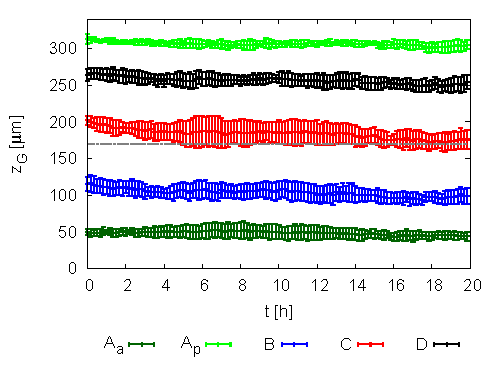
\includegraphics[width=0.48\textwidth]{Figures/FigureRestoringForcePinnedCN15-Center.pdf}
  }
  \subfigure{
    \label{Fig-SI-RestoringForcePinnedFromBoundary}
    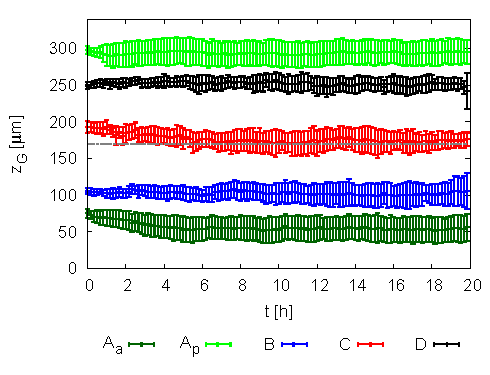
\includegraphics[width=0.48\textwidth]{Figures/FigureRestoringForcePinnedCN15-Boundary.pdf}
  }
\caption{\textbf{Perturbed trajectories are restored to their origin at optimal NN repression strength.}
    Shown are averaged time traces of the copy number center-of-masses $z_G$ for the five domains
    of the stable pattern (${\rm \GA}_a$ = anterior \GA domain, ${\rm \GA}_p$ = posterior \GA domain) at $\kappa=\kappa_{opt}$
    for two different perturbations: 
    \mysubref{Fig-SI-RestoringForcePinnedFromCenter} ``\GC expansion'', i.e. prolongation of the 
    central \GC domain by $\Delta=8$ nuclei into the posterior
    and \mysubref{Fig-SI-RestoringForcePinnedFromBoundary} ``\GA expansion'', 
    i.e. prolongation of the anterior \GA domain by $\Delta=8$ nuclei towards the center of the embryo.
    The gray-dashed line marks the center of the system.
    In both cases we observe a restoration of the metastable state on a timescale $\lesssim 10~\unit{h}$.\\
  \label{Fig-SI-RestoringForcePinned}
}
\end{figure}

\section{Estimation of phase space diffusion coefficient from overdamped Langevin dynamics}
\label{Sec-SI-OverdampedLangevin} \index{overdamped Langevin dynamics}
%\TODO{Rewrite this in vector notation}

Let $f(X,Y,t)$ be a twice differentiable real function depending on a two-dimensional diffusion-drift processes $\vekA X=(X,Y)$ and time $t$ (explicitly).
In the overdamped Langevin limit, i.e. assuming that the displacements of the random walker are goverened only
by forces that stem from an underlying force field and by Gaussian noise, and that its accelerations and inertia are negligible,
we can describe this random processes via
\begin{align}
d\vekA X & = \vekA v dt + \sigma d\vekA W
\end{align}
where $\vekA W$ is a (two-dimensional) Wiener processes and $\vekA v = (v_X, v_Y)$ a (local) drift velocity resulting from the potential forces.

\pagebreak
\noindent We then can calculate the differential of $f$ with \textsc{It\={o}}'s Lemma (as a generalization of Taylor expansion) as follows:
\newcommand{\pder}[2]{\frac{\partial #1}{\partial #2}}
\newcommand{\pderII}[2]{\frac{\partial^2 #1}{\partial #2^2}}
\begin{align}
 df(X,Y,t) & = \sigma \pder{f}{X} dW_X + \sigma \pder{f}{Y} dW_Y  \nn\\
	   & \quad + \left[ \pder{f}{t} + v_X \pder{f}{X} + v_Y \pder{f}{Y}
			    + \frac{\sigma^2}{2}\pderII{f}{X} + \frac{\sigma^2}{2}\pderII{f}{Y} 
			    + \zeta \sigma^2 \frac{\partial^2 f}{\partial X \partial Y} \right] dt	\nn\\
\end{align}
Here $\zeta$ measures the correlation between $X$ and $Y$.

In order to apply this general formula to the specific diffusion-drift problem for the phase space coordinates $(\lambda_{AC}, \lambda_{BD})$ defined in the main text eq. (2), we assign for brevity $\lambda_x = \lambda_{AC}$ and $\lambda_y = \lambda_{BD}$, and then
we set $X=\lambda_x, Y=\lambda_y$ and $f(X,Y,t)=f(\lambda_x,\lambda_y)=(\lambda_x-\lambda_{x_0})^2 + (\lambda_y-\lambda_{y_0})^2 \equiv \Delta\lambda^2$
(the squared displacement function).

It\={o}'s Lemma now reads (note that the time and mixed derivatives vanish):
\begin{align}
 d (\Delta\lambda^2) &= d \left[ (\Delta\lambda_x)^2 + (\Delta\lambda_y)^2 \right] = d \left[ (\lambda_x-\lambda_{x_0})^2 + (\lambda_y-\lambda_{y_0})^2 \right] \nn\\
		     &\simeq 2(\lambda_x-\lambda_{x_0}) (v_{\lambda_x} dt + \sigma dW_x) + 2(\lambda_y-\lambda_{y_0}) (v_{\lambda_y} dt + \sigma dW_y) \nn\\
		     & \quad + \frac{\sigma^2}{2} 2 dt + \frac{\sigma^2}{2} 2 dt
\end{align}

%%%%%%%%%%%%%%%%%
%%% FIGURE S6 %%%
%%%%%%%%%%%%%%%%%
\begin{figure}[H]
  \centering
  \subfigure[][]{
    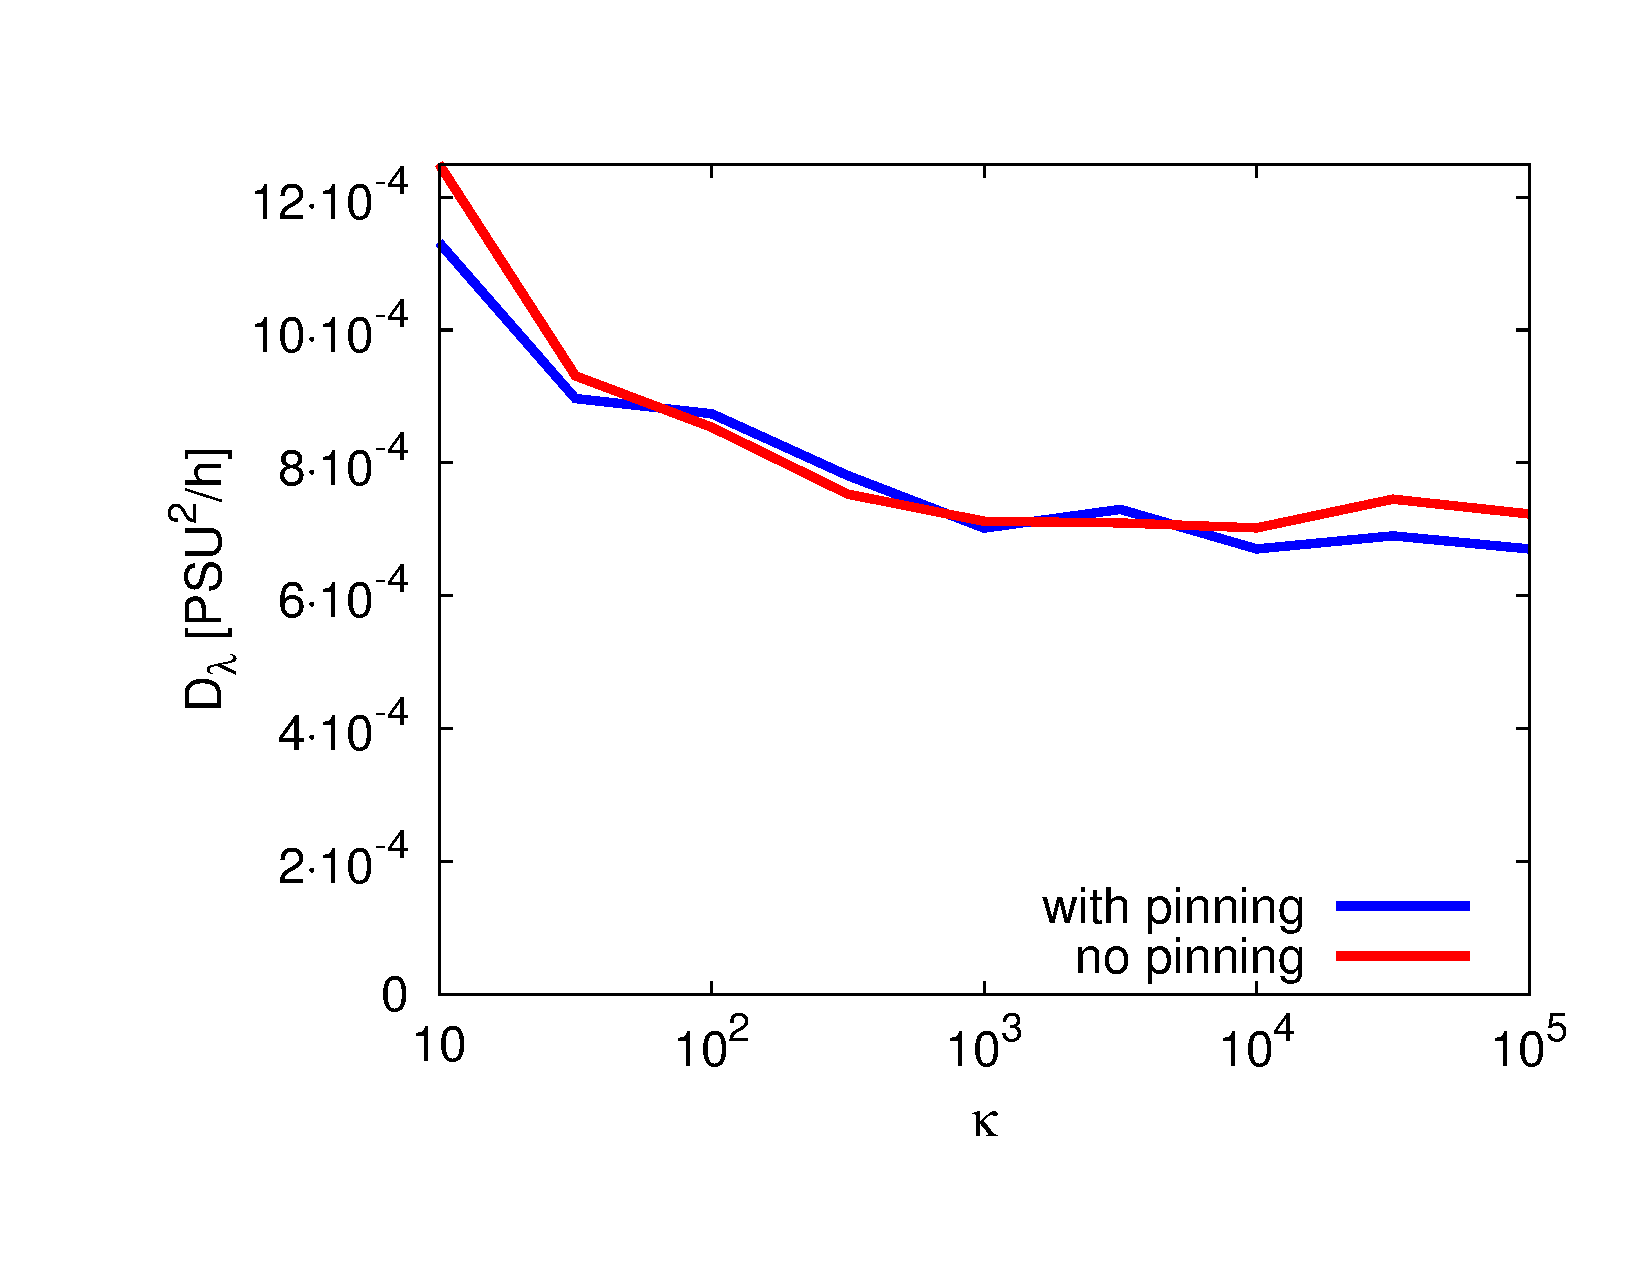
\includegraphics[width=0.6\textwidth]{Figures-SI/FigureDiffusionCoefficients.pdf}
    \label{Fig-GG-SI-DiffusionCoefficients}
  }
  \subfigure[][]{
    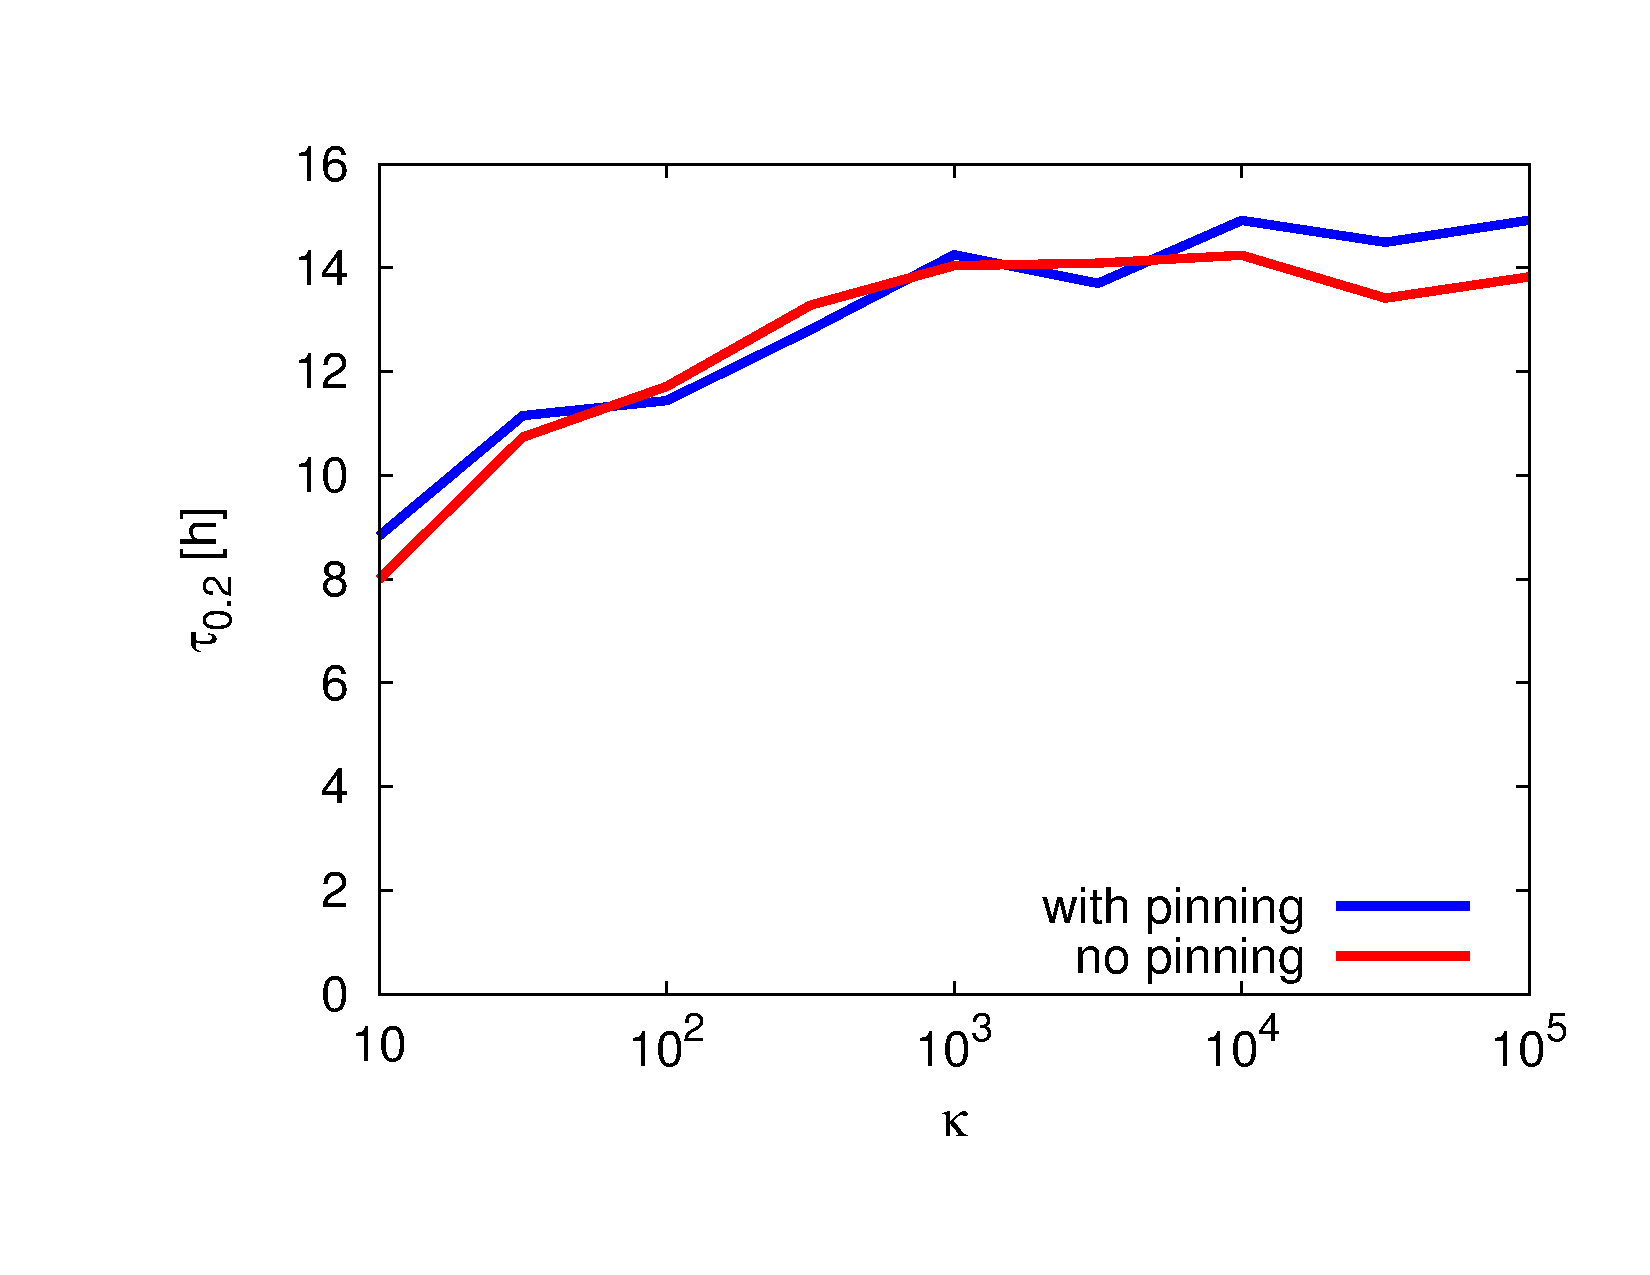
\includegraphics[width=0.6\textwidth]{Figures-SI/FigureDiffusionTimes.pdf}
    \label{Fig-GG-SI-DiffusionTimes}
  }  
  \caption{\textbf{Average phase space diffusion coefficients as a function of $\kappa$.} 
  \mysubref{Fig-GG-SI-DiffusionCoefficients} The diffusion coefficient of phase space trajectories in the $(\lambda_x, \lambda_y) = (\lambda_{AC}, \lambda_{BD})$ space are obtained from the overdamped Langevin analysis, see section \ref{Sec-SI-OverdampedLangevin}. The diffusion coefficients are averaged over the phase space region $R_P=[0.3,0.4]^2$, which is part of the diffusive plateau, for different repression strength ratios $\kappa$. The PSU stands for the phase space units.
  \mysubref{Fig-GG-SI-DiffusionTimes} The resulting approximate diffusion times from the phase space region of the five-stripe relaxed patterns, towards the edge of the diffusive plateau as a function of $\kappa$, assuming a distance of $0.2$ PSU for the initial phase space distance to the edge. The edge of diffusive plateau is defined as a region of $(\lambda_{AC}, \lambda_{BD})$ from which the states are quickly absorbed into the regions with one the domains lost.
  \label{Fig-GG-SI-Diffusion}
}
\end{figure}

\pagebreak
To relate the above formula to the displacements sampled in our simulations with a fixed acquisition time interval $\Delta t$
we shall integrate the infinitesimal contributions over this interval.
At the same time we take the ensemble average to account for the averaging of independent samples, which causes the
Gaussian terms $\sigma dW_x$ and $\sigma dW_y$ to vanish.
We further assume that, to a good approximation, the drift velocities and diffusion coefficients are constant 
over the time interval $\Delta t$ and diffusion isotropic in $\lambda_x$ and $\lambda_y$ direction,
i.e. $D_{\lambda_x}=D_{\lambda_y}=D_\lambda(\vekA{\lambda})$.
%In practice this assumption is valid if $\Delta t$ is chosen large enough to ensure that the random walk transits
%from the initial ballistic to the subsequent diffusive regime,
%yet significantly smaller than the average time that it takes to travel a distance comparable to the system size.
Finally, using $\sigma = \sqrt{2 D_\lambda}$, we obtain:
\begin{align}
 \avg{\Delta\lambda^2} &= \avg{\int_{\Delta t} d(\Delta\lambda^2) } 	\nn\\
		       &= \avg{\int_{0}^{\Delta t} 2 \underbrace{\left[ \lambda_x(t) - \lambda_{x}(0) \right]}_{\simeq\avg{v_{\lambda_x}}t} \underbrace{v_{\lambda_x}}_{\simeq \avg{v_{\lambda_x}}} dt}
			+ \avg{\int_{0}^{\Delta t} 2 \underbrace{\left[ \lambda_y(t) - \lambda_{y}(0) \right]}_{\simeq\avg{v_{\lambda_y}}t} \underbrace{v_{\lambda_y}}_{\simeq \avg{v_{\lambda_y}}} dt} \nn\\
		       &\quad + \avg{\int_0^{\Delta t} 4D_\lambda dt} 
			      + \int_{\Delta t} \underbrace{\avg{2\Delta\lambda_x\sigma dW_x}}_{0} + \int_{\Delta t} \underbrace{\avg{2\Delta\lambda_y\sigma dW_y } }_{0} \nn\\
		       &\simeq \avg{ \avg{v_{\lambda_x}}^2 \int_{0}^{\Delta t} 2t dt} + \avg{ \avg{v_{\lambda_y}}^2 \int_{0}^{\Delta t} 2t dt}
			  + 4 \avg{D_\lambda} \Delta t										\nn\\
		       &\simeq \avg{v_{\lambda_x}\Delta t}^2 + \avg{v_{\lambda_y}\Delta t}^2 + 4 \avg{D_\lambda} \Delta t	\nn\\
		       &= \avg{\Delta{\lambda_x}}^2 + \avg{\Delta{\lambda_y}}^2 + 4 \avg{D_\lambda} \Delta t
\end{align}

The final result shows that, knowing the average displacements $\avg{\Delta{\lambda_x}}$ and $\avg{\Delta{\lambda_x}}$ and average
squared displacements $\avg{\Delta\lambda^2}$ at $\vekA{\lambda}$, we can compute
the average diffusion coefficient $\avg{D_\lambda}(\vekA{\lambda})$ via:
\begin{align}
 \avg{D_\lambda}(\vekA{\lambda}) &= \frac{1}{4\Delta t} \left[ \avg{\Delta\lambda^2}(\vekA{\lambda}) - \left( \avg{\Delta{\lambda_x}}^2(\vekA{\lambda}) + \avg{\Delta{\lambda_y}}^2(\vekA{\lambda}) \right)\right]
				 = \frac{1}{4\Delta t} \mathcal{V}_{\avg{\lambda}}(\vekA{\lambda})
\end{align}
The bracket term containing the first moments corrects the mean squared displacement for the contributions coming from the deterministic drift
and tends to zero as the process becomes purely diffusive.

The results of this analysis applied to our simulated systems are shown in Fig.~\ref{Fig-GG-SI-Diffusion}, where we plot the diffusion coefficients and the resulting expected diffusion times to the edge of the basin of initial patterns as a function of our main parameter, the repression strength ratio $\kappa$.



%%%%% TODO: WE PUT THIS BACK INTO THE NEXT VERSION, TOMEK HAS
%%%%% TO FINISH RE-MAKING THE PLOTS
\begin{comment}
\section{Supplementary velocity field figures}
Figures \ref{Fig-GG-SI-VelocitiesPinnedOptimum}, \ref{Fig-GG-SI-VelocitiesPinnedKappa1000}, \ref{Fig-GG-SI-VelocitiesUnpinnedOptimum} and \ref{Fig-GG-SI-VelocitiesUnpinnedKappa1000}
show phase space velocity fields and trajectories starting from perturbed initial conditions for three different projections of the reaction coordinates,
for the following cases:
\begin{itemize}
\item for the repression strength ratio $\kappa\simeq31.6$ that optimizes pattern stability with pinning, see Fig. \ref{Fig-GG-SI-VelocitiesPinnedOptimum},
\item for weaker NN repression strength $\kappa=1000$ with pinning, see Fig. \ref{Fig-GG-SI-VelocitiesPinnedKappa1000},
\item for the optimal repression strength ratio $\kappa=100$ that optimizes pattern stability without pinning, see Fig. \ref{Fig-GG-SI-VelocitiesUnpinnedOptimum},
\item for weaker NN repression strength $\kappa=1000$ without pinning, see Fig. \ref{Fig-GG-SI-VelocitiesUnpinnedKappa1000}.
\end{itemize}


\newcommand{\GGSIVelocityFigureScale}{0.33\textwidth}
% \renewcommand{\subfigcapskip}{-12pt}
% \renewcommand{\subfigcapmargin}{-12pt}
%%%%%%%%%%%%%%%%%
%%% FIGURE S2 %%%
%%%%%%%%%%%%%%%%%
\begin{figure}[H]
  \centering
  \subfigure[][]{
    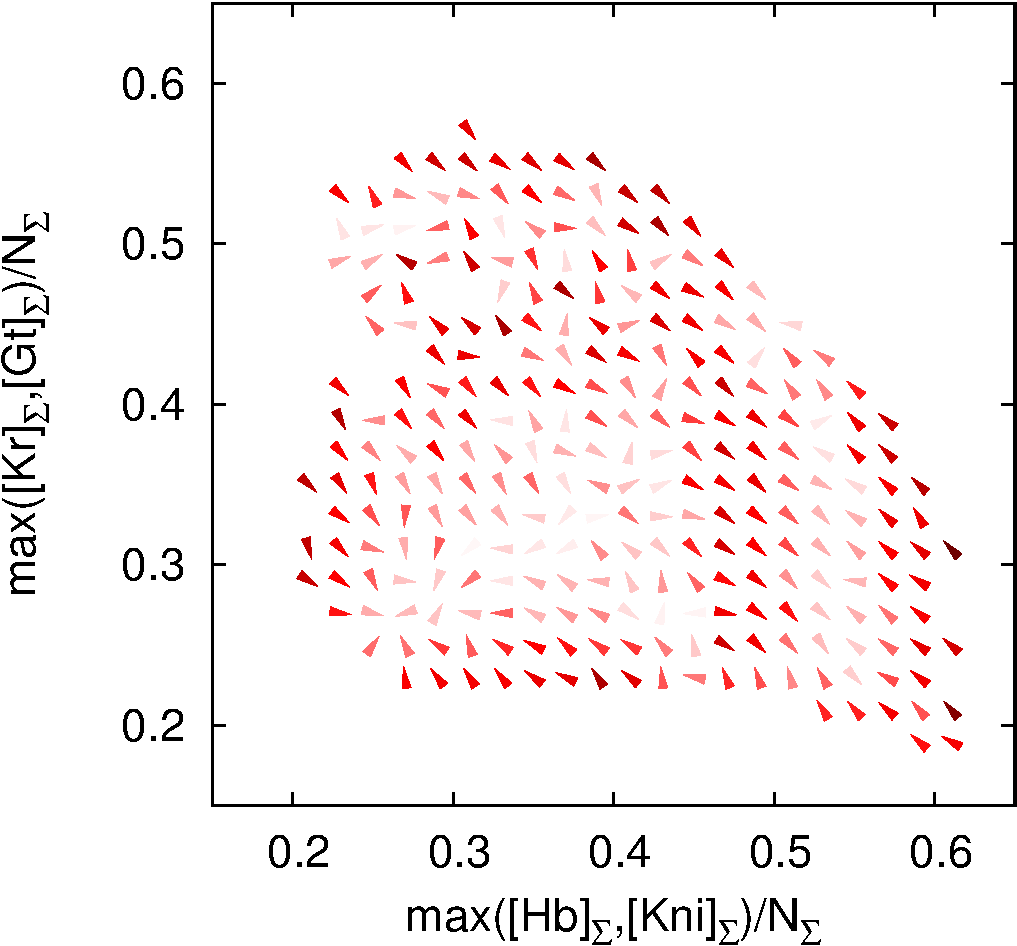
\includegraphics[height=\GGSIVelocityFigureScale]{Figures-SI/FigureVelocitiesPinnedOptimum.pdf}
    \label{Fig-GG-SI-VelocitiesPinnedOptimum-Std}
  }
  \subfigure[][]{
    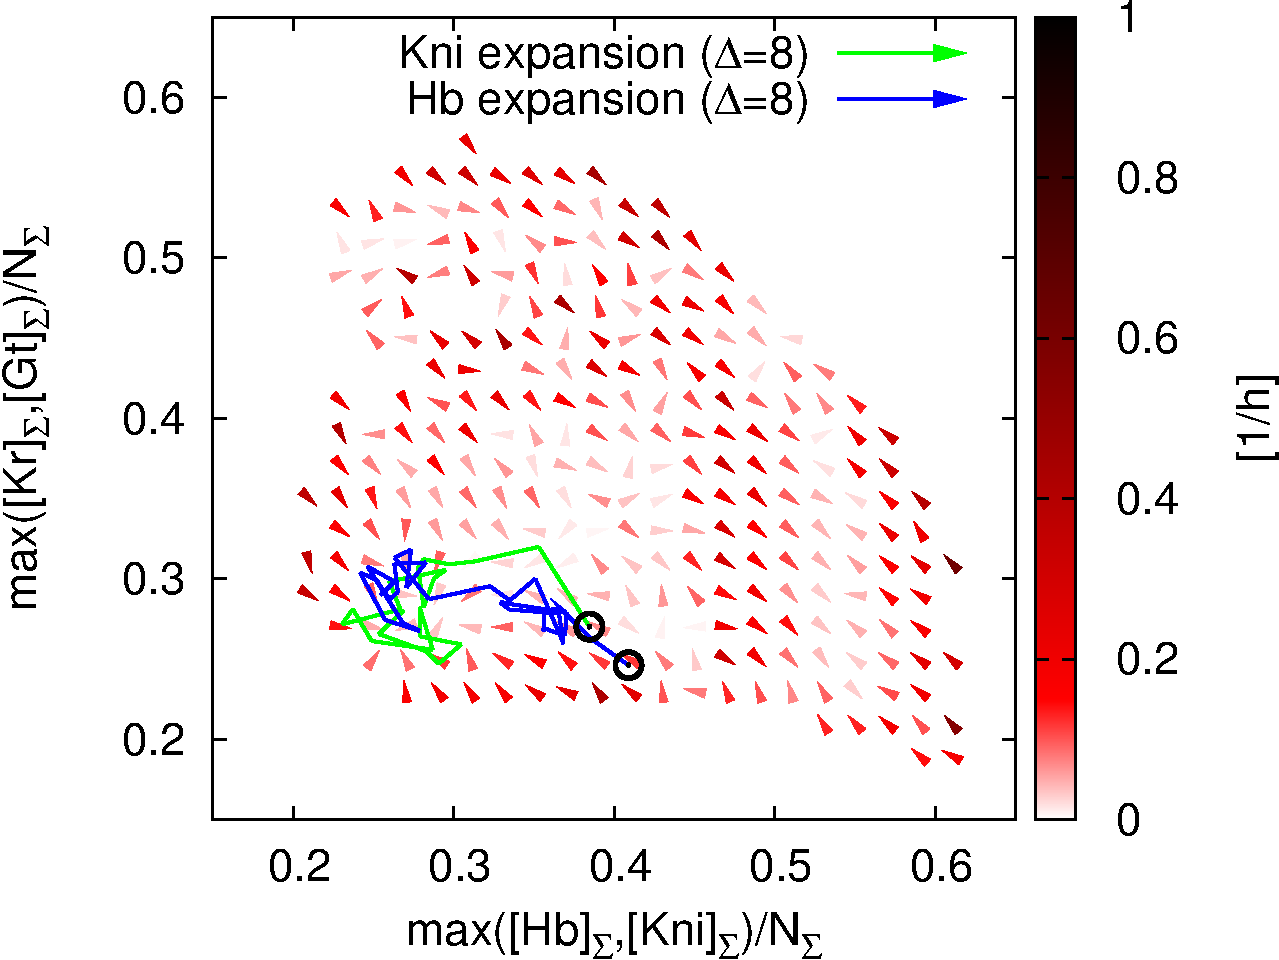
\includegraphics[height=\GGSIVelocityFigureScale]{Figures-SI/FigureVelocitiesPinnedOptimum-Relax.pdf}
    \label{Fig-GG-SI-VelocitiesPinnedOptimum-Std-Relax}
  }\\
  \subfigure[][]{
    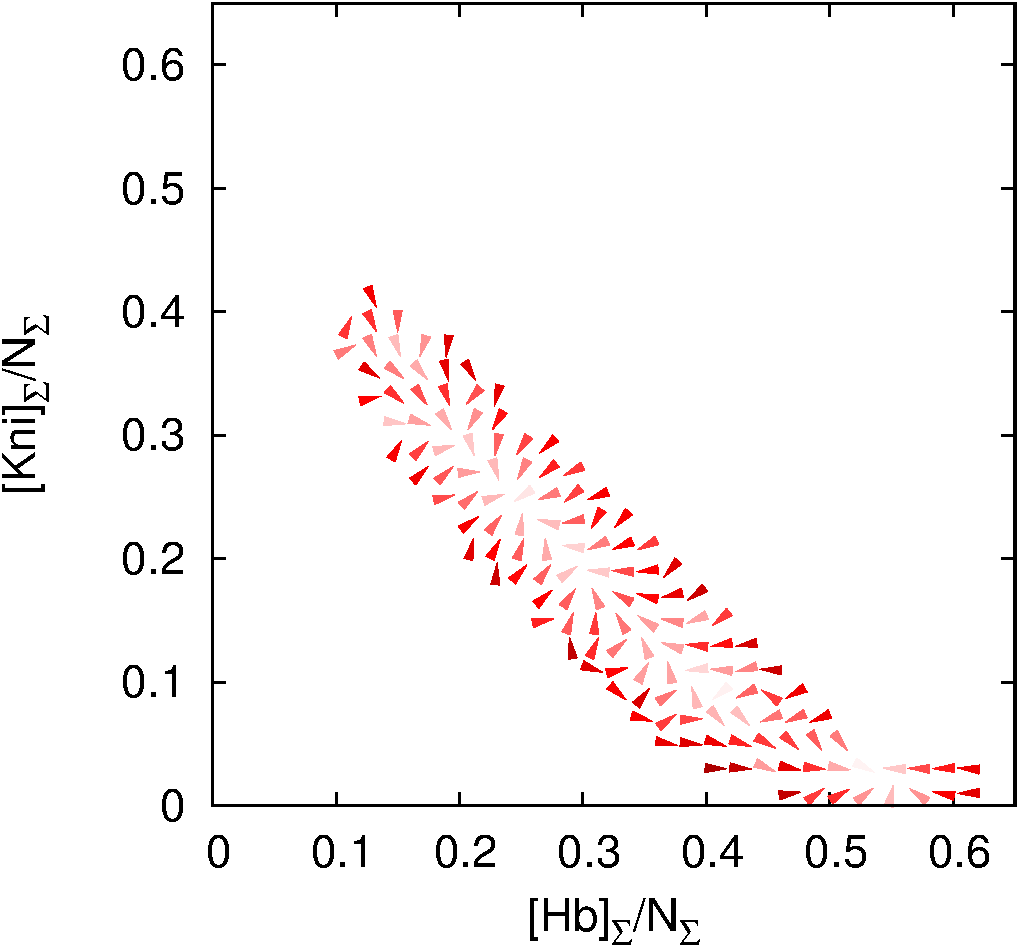
\includegraphics[height=\GGSIVelocityFigureScale]{Figures-SI/FigureVelocitiesPinnedOptimumHbKni.pdf}
    \label{Fig-GG-SI-VelocitiesPinnedOptimum-HbKni}
  }
  \subfigure[][]{
    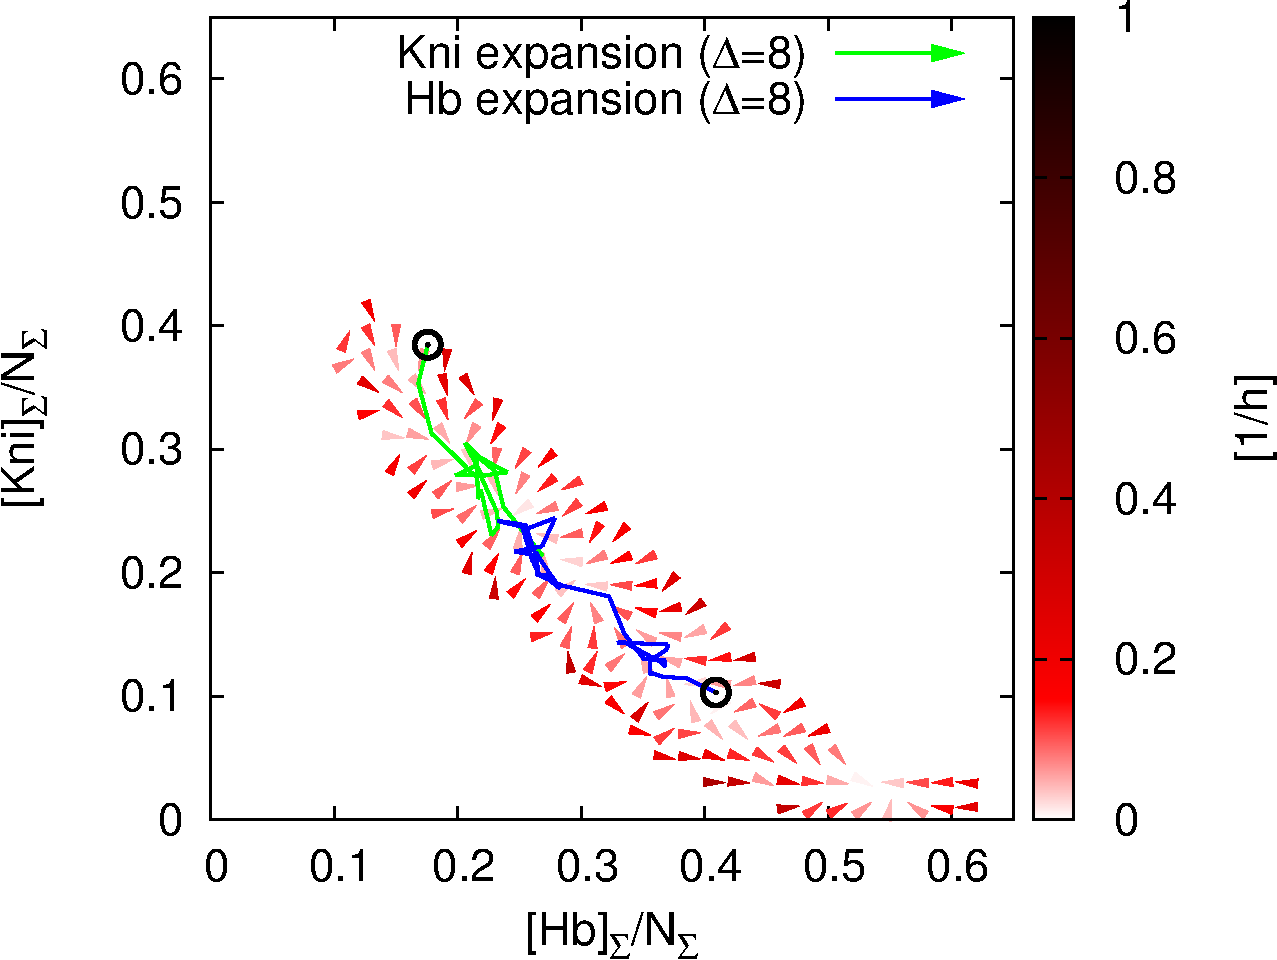
\includegraphics[height=\GGSIVelocityFigureScale]{Figures-SI/FigureVelocitiesPinnedOptimumHbKni-Relax.pdf}
    \label{Fig-GG-SI-VelocitiesPinnedOptimum-HbKni-Relax}
  }\\
  \subfigure[][]{
    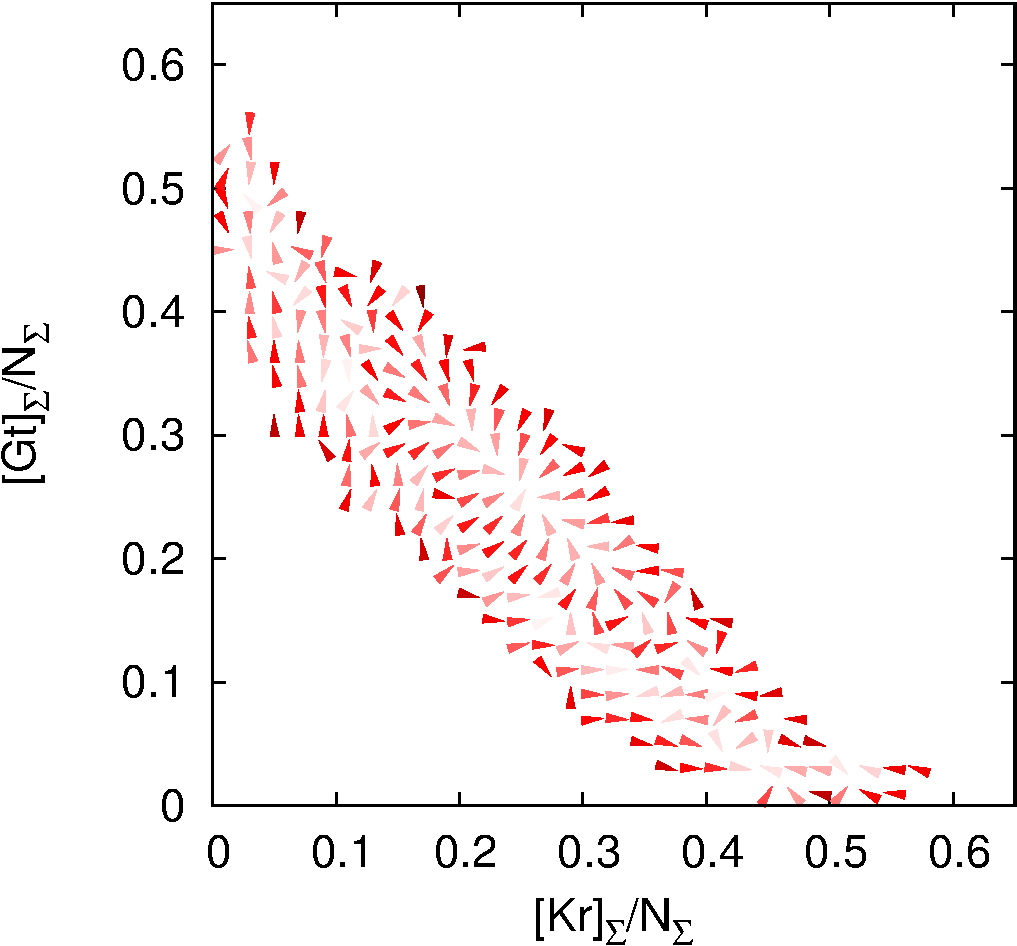
\includegraphics[height=\GGSIVelocityFigureScale]{Figures-SI/FigureVelocitiesPinnedOptimumKrGt.pdf}
    \label{Fig-GG-SI-VelocitiesPinnedOptimum-KrGt}
  }
  \subfigure[][]{
    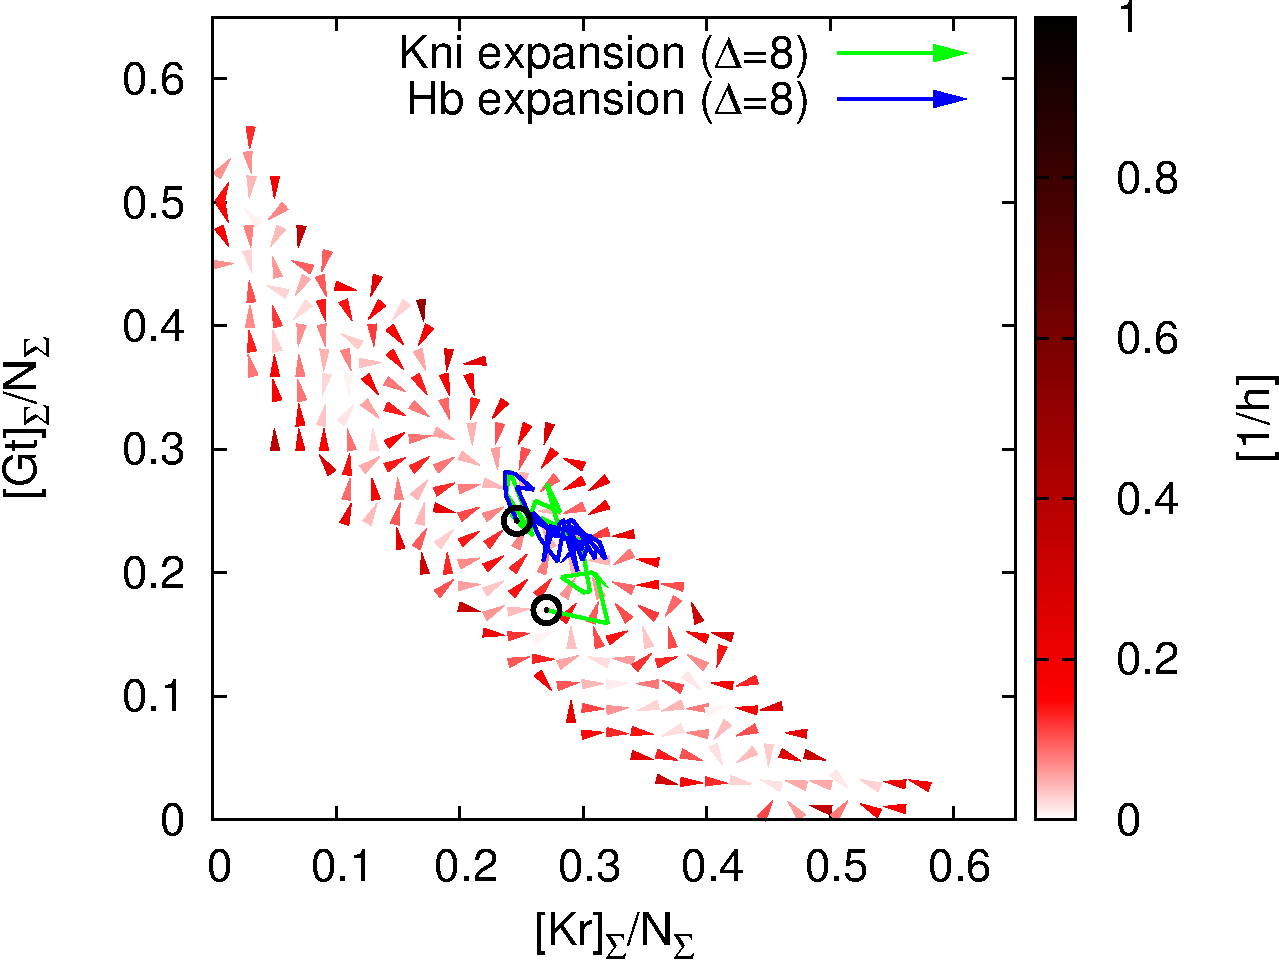
\includegraphics[height=\GGSIVelocityFigureScale]{Figures-SI/FigureVelocitiesPinnedOptimumKrGt-Relax.pdf}
    \label{Fig-GG-SI-VelocitiesPinnedOptimum-KrGt-Relax}
  }
  \caption{\textbf{Average phase space velocities for the maximally stable system ($\kappa\simeq31.6$) with pinning.}
      Left plots (A, C, E) show local average phase space velocities, right plots (B, D, F) additionally show 
      example trajectories for the two types of perturbations considered in the restoration experiments.
      Starting points are marked by black bullets.
      %Velocity magnitude is denoted by color on a range from $0$ (white) to $1.0/\mathrm{h}$ (black) with bright red at $0.15/\mathrm{h}$.
      \TODO{Adapt gene names to (A,B,C,D) scheme !!!}
  \label{Fig-GG-SI-VelocitiesPinnedOptimum}
 }
\end{figure}

%%%%%%%%%%%%%%%%%
%%% FIGURE S3 %%%
%%%%%%%%%%%%%%%%%
\begin{figure}[H]
  \centering  
  \subfigure[][]{
    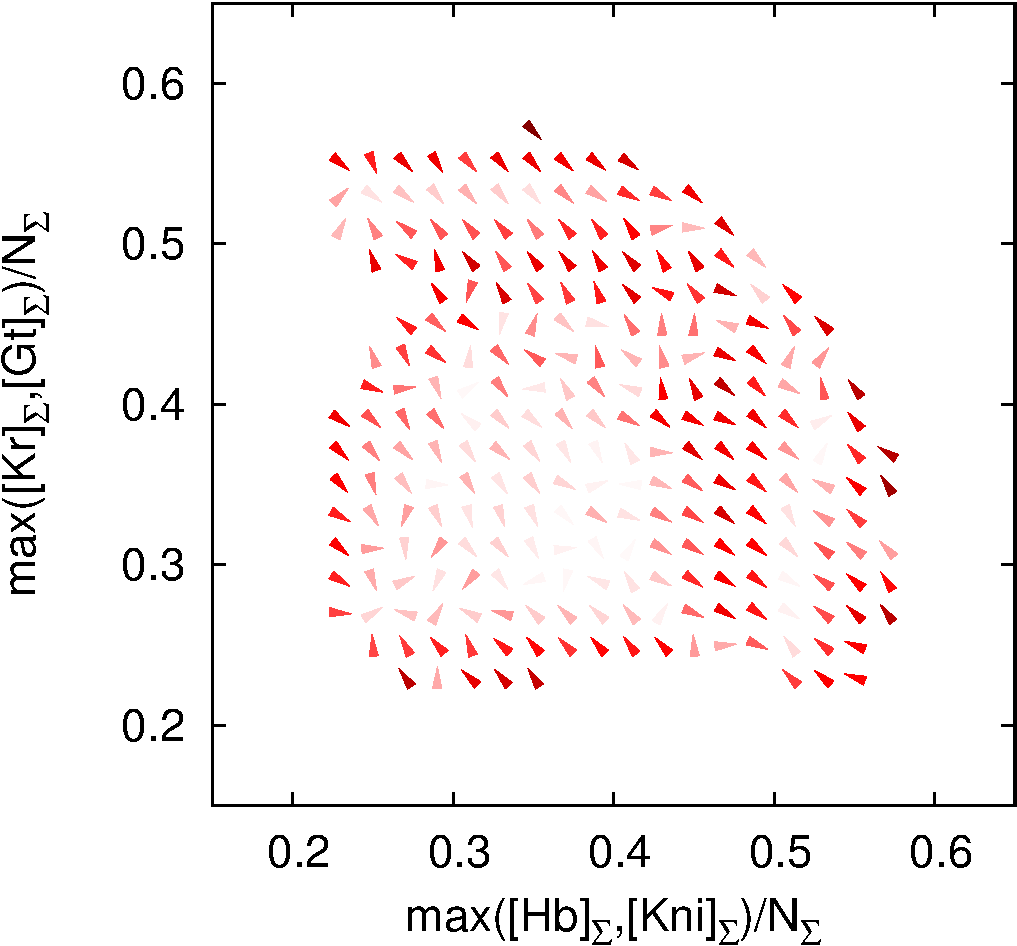
\includegraphics[height=\GGSIVelocityFigureScale]{Figures-SI/FigureVelocitiesPinnedKappa1000.pdf}
    \label{Fig-GG-SI-VelocitiesPinnedKappa1000-Std}
  }
  \subfigure[][]{
    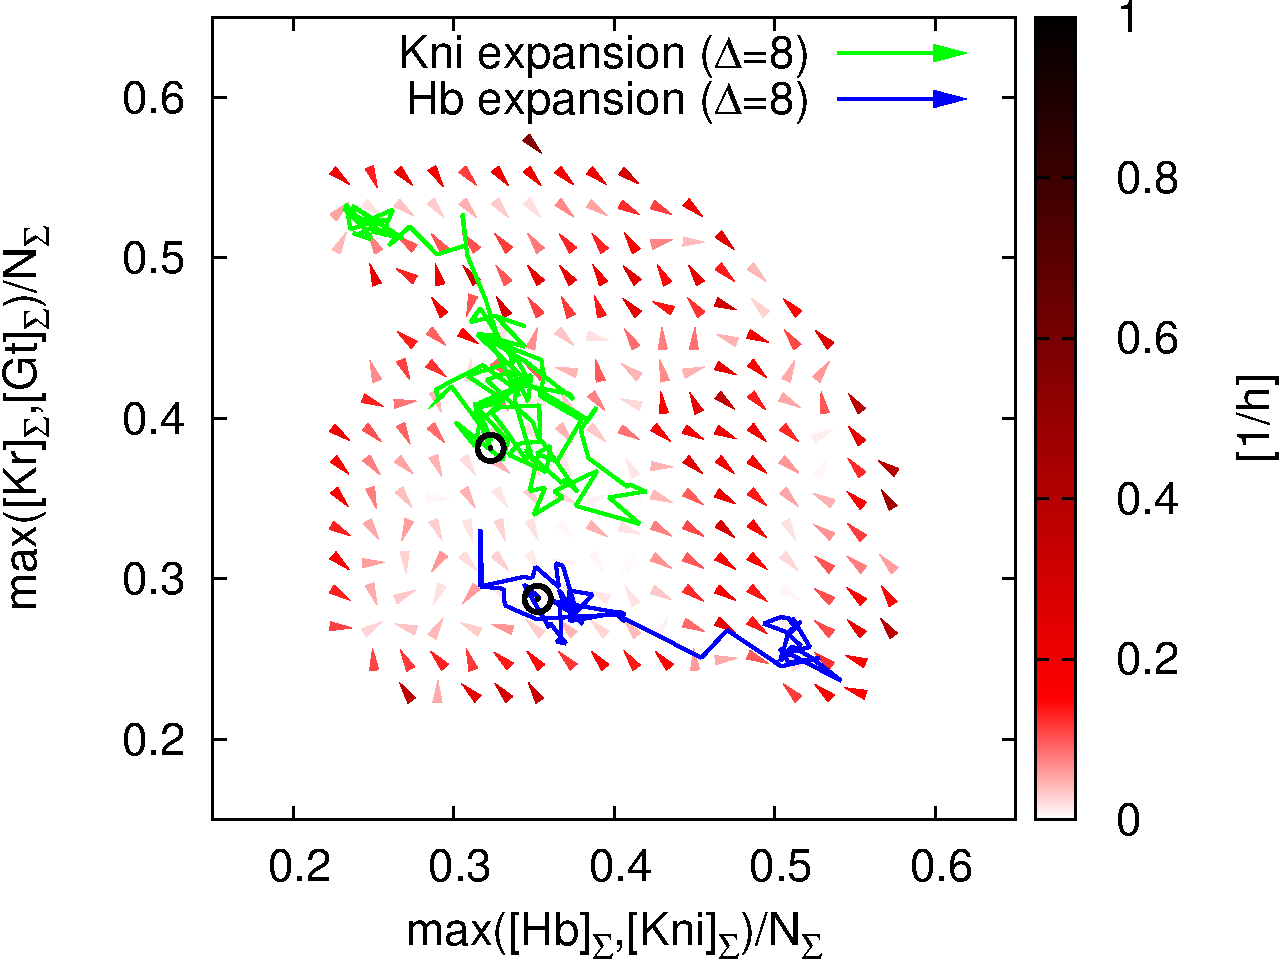
\includegraphics[height=\GGSIVelocityFigureScale]{Figures-SI/FigureVelocitiesPinnedKappa1000-Relax.pdf}
    \label{Fig-GG-SI-VelocitiesPinnedKappa1000-Std-Relax}
  }\\
  \subfigure[][]{
    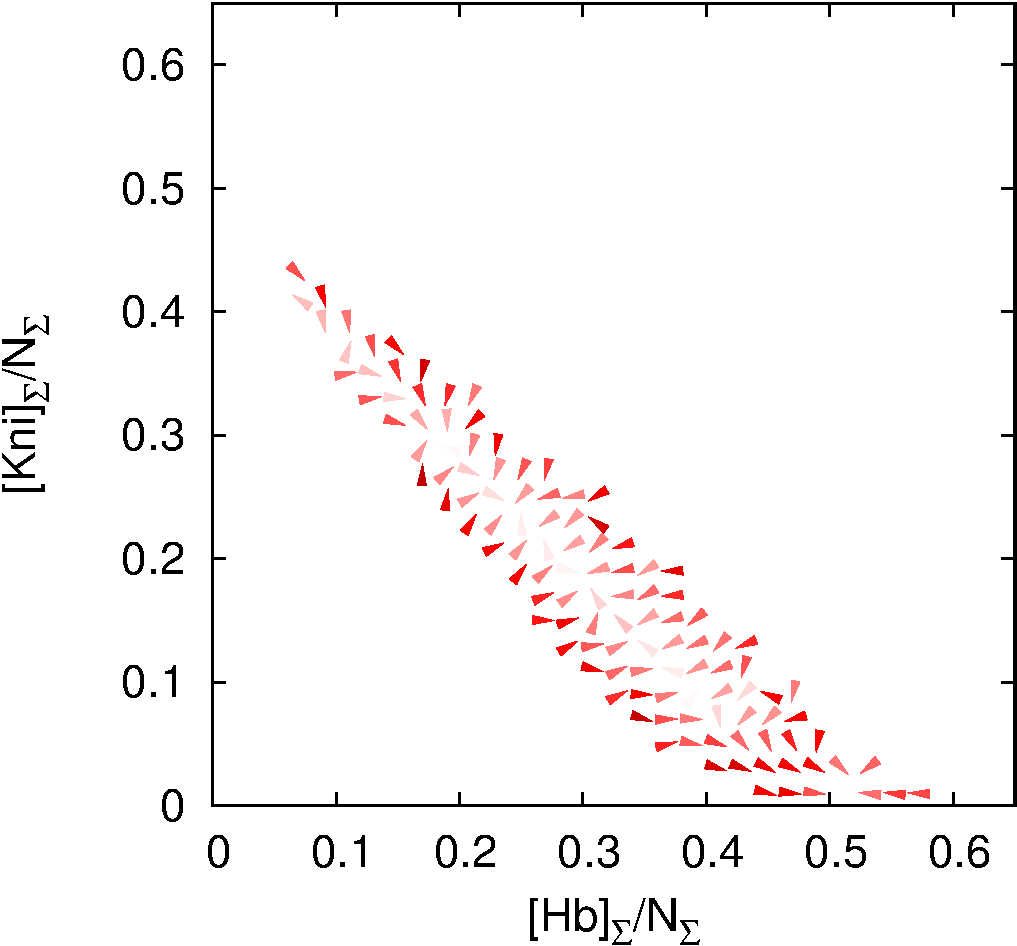
\includegraphics[height=\GGSIVelocityFigureScale]{Figures-SI/FigureVelocitiesPinnedKappa1000HbKni.pdf}
    \label{Fig-GG-SI-VelocitiesPinnedKappa1000-HbKni}
  }
  \subfigure[][]{
    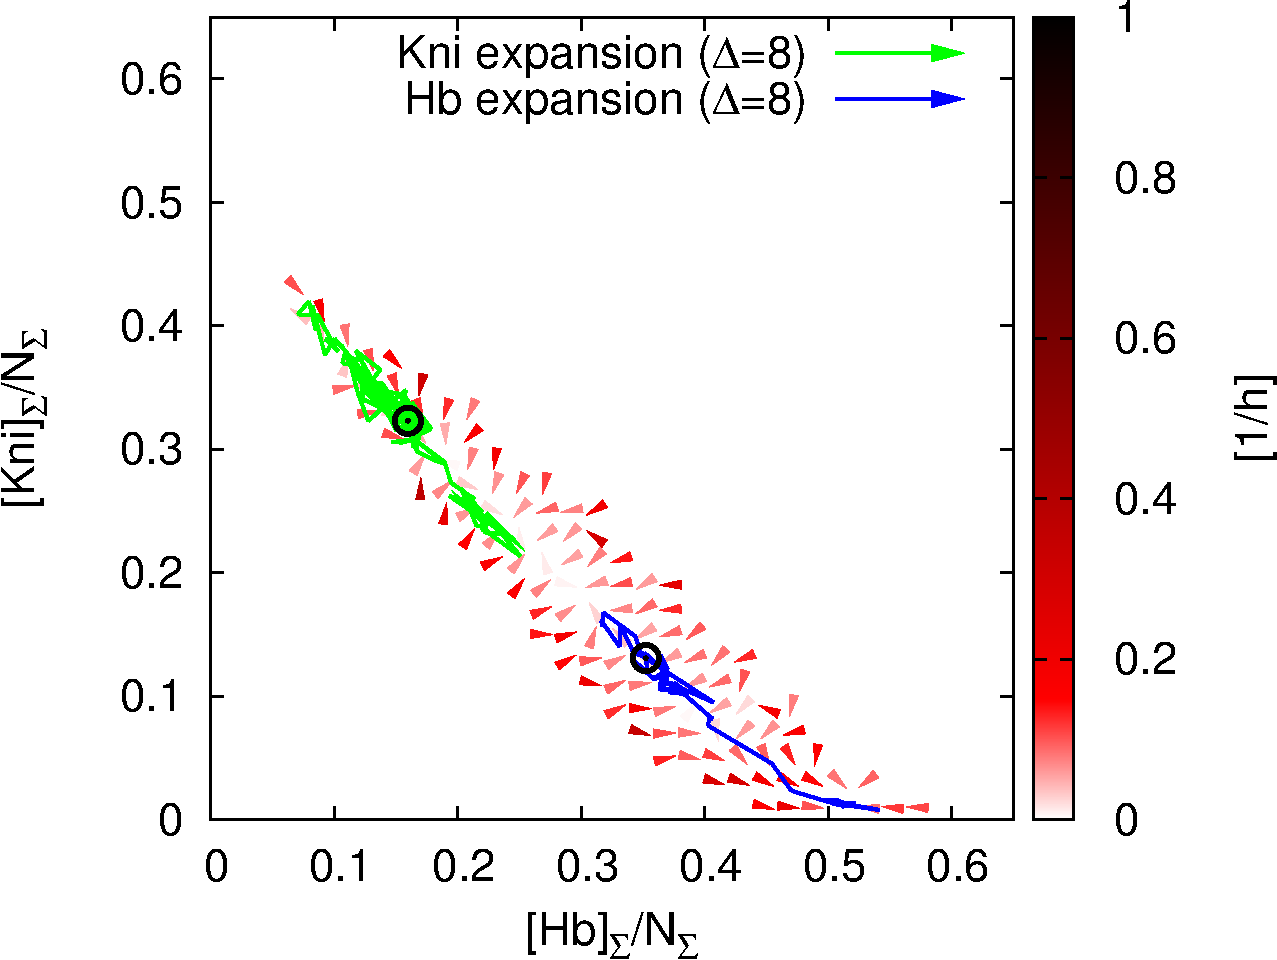
\includegraphics[height=\GGSIVelocityFigureScale]{Figures-SI/FigureVelocitiesPinnedKappa1000HbKni-Relax.pdf}
    \label{Fig-GG-SI-VelocitiesPinnedKappa1000-HbKni-Relax}
  }\\
  \subfigure[][]{
    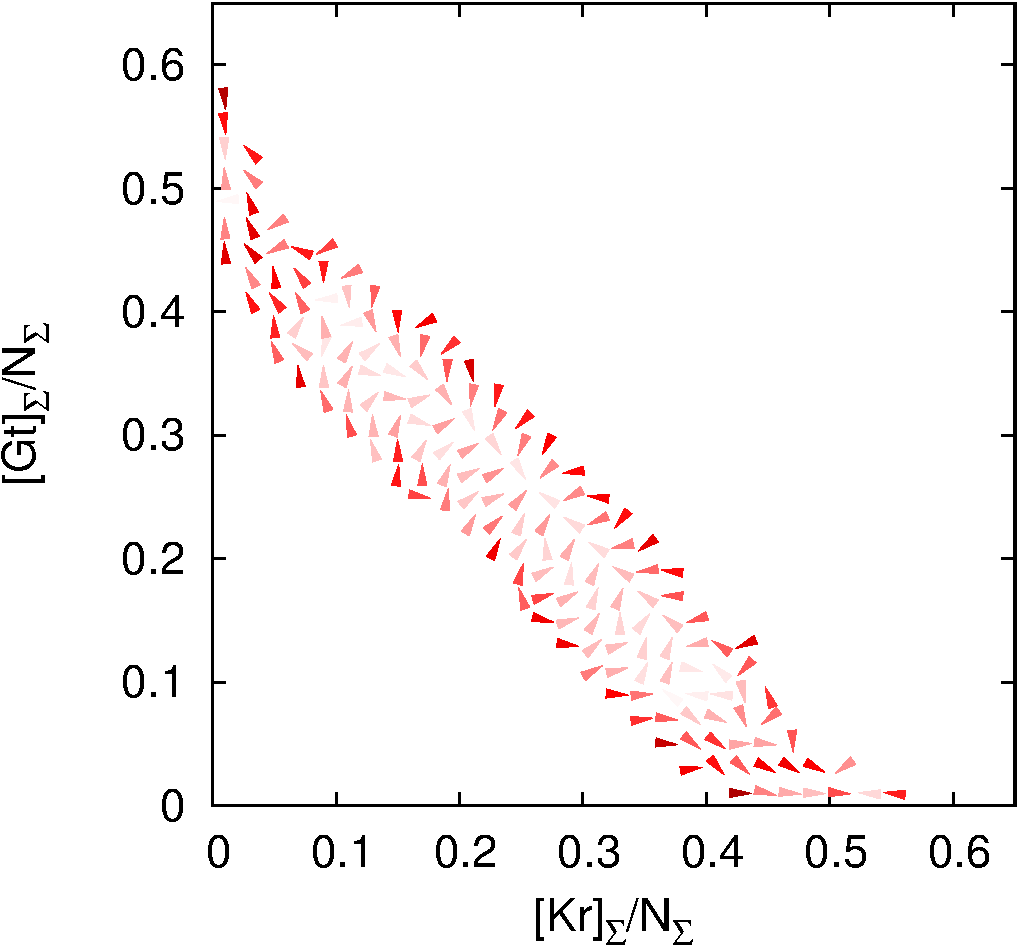
\includegraphics[height=\GGSIVelocityFigureScale]{Figures-SI/FigureVelocitiesPinnedKappa1000KrGt.pdf}
    \label{Fig-GG-SI-VelocitiesPinnedKappa1000-KrGt}
  }
  \subfigure[][]{
    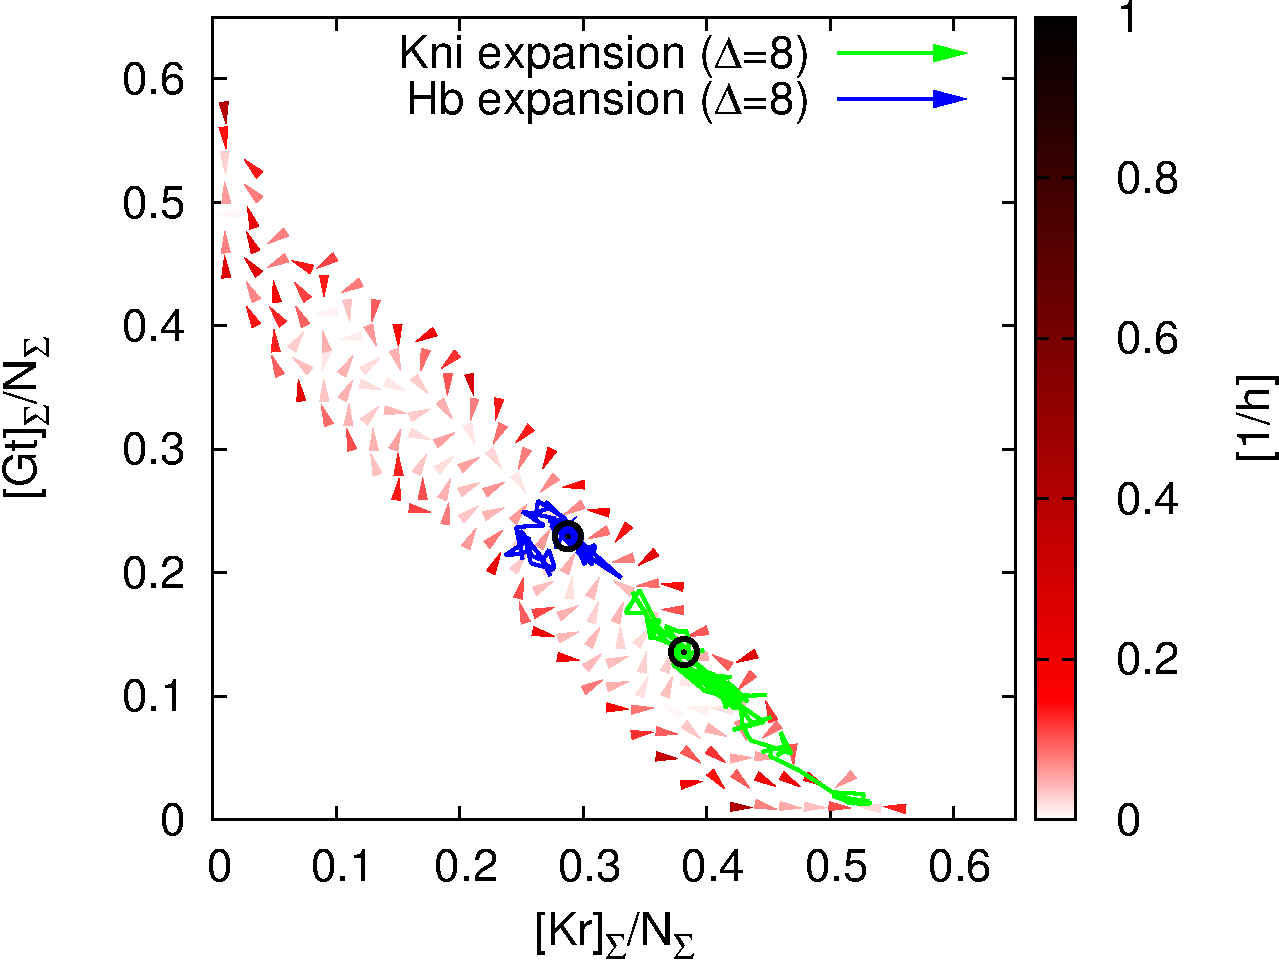
\includegraphics[height=\GGSIVelocityFigureScale]{Figures-SI/FigureVelocitiesPinnedKappa1000KrGt-Relax.pdf}
    \label{Fig-GG-SI-VelocitiesPinnedKappa1000-KrGt-Relax}
  }
  \caption{\textbf{Average phase space velocities for weaker NN interaction ($\kappa=1000$) in the system with pinning.}
      Left plots (A, C, E) show local average phase space velocities, right plots (B, D, F) additionally show 
      example trajectories for the two types of perturbations considered in the restoration experiments.
      Starting points are marked by black bullets.
      %Velocity magnitude is denoted by color on a range from $0$ (white) to $1.0/\mathrm{h}$ (black) with bright red at $0.15/\mathrm{h}$.
      \TODO{Adapt gene names to (A,B,C,D) scheme !!!}
    \label{Fig-GG-SI-VelocitiesPinnedKappa1000}
    }
\end{figure}

%%%%%%%%%%%%%%%%%
%%% FIGURE S4 %%%
%%%%%%%%%%%%%%%%%
\begin{figure}[H]
  \centering
  \subfigure[][]{
    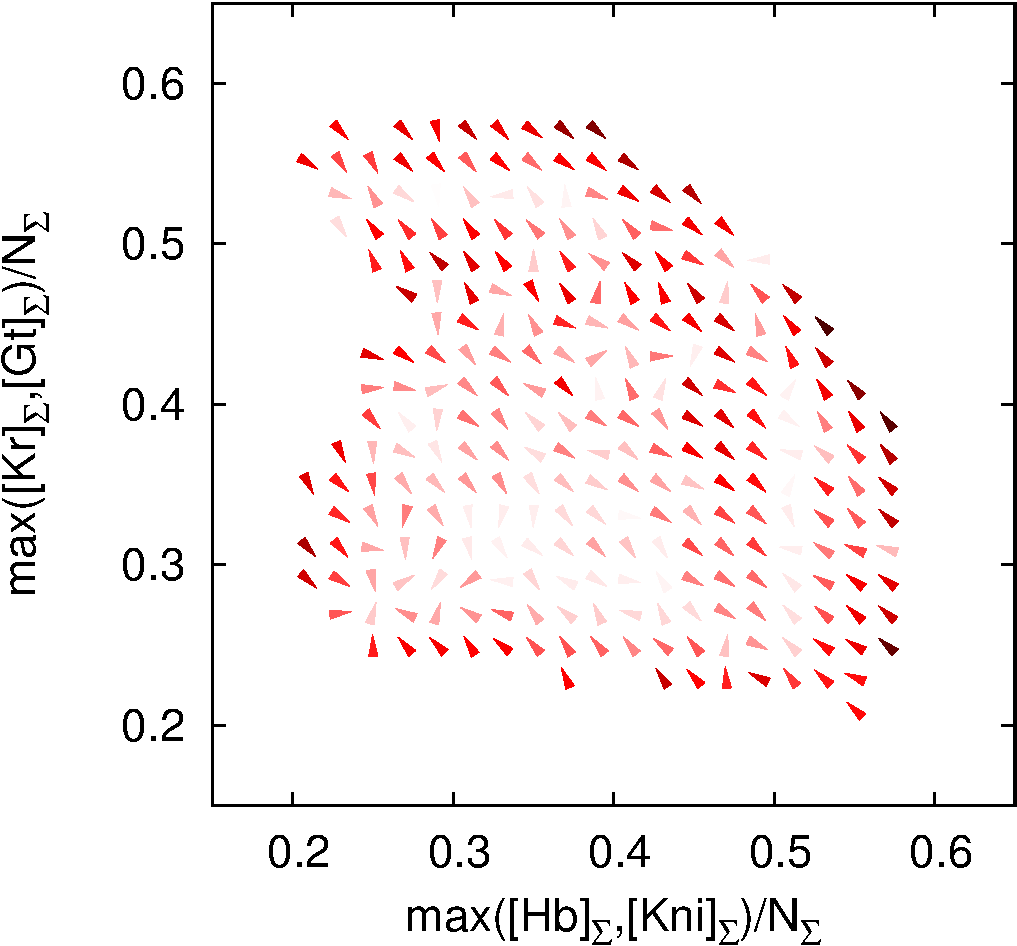
\includegraphics[height=\GGSIVelocityFigureScale]{Figures-SI/FigureVelocitiesUnpinnedOptimum.pdf}
    \label{Fig-GG-SI-VelocitiesUnpinnedOptimum-Std}
  }
  \subfigure[][]{
    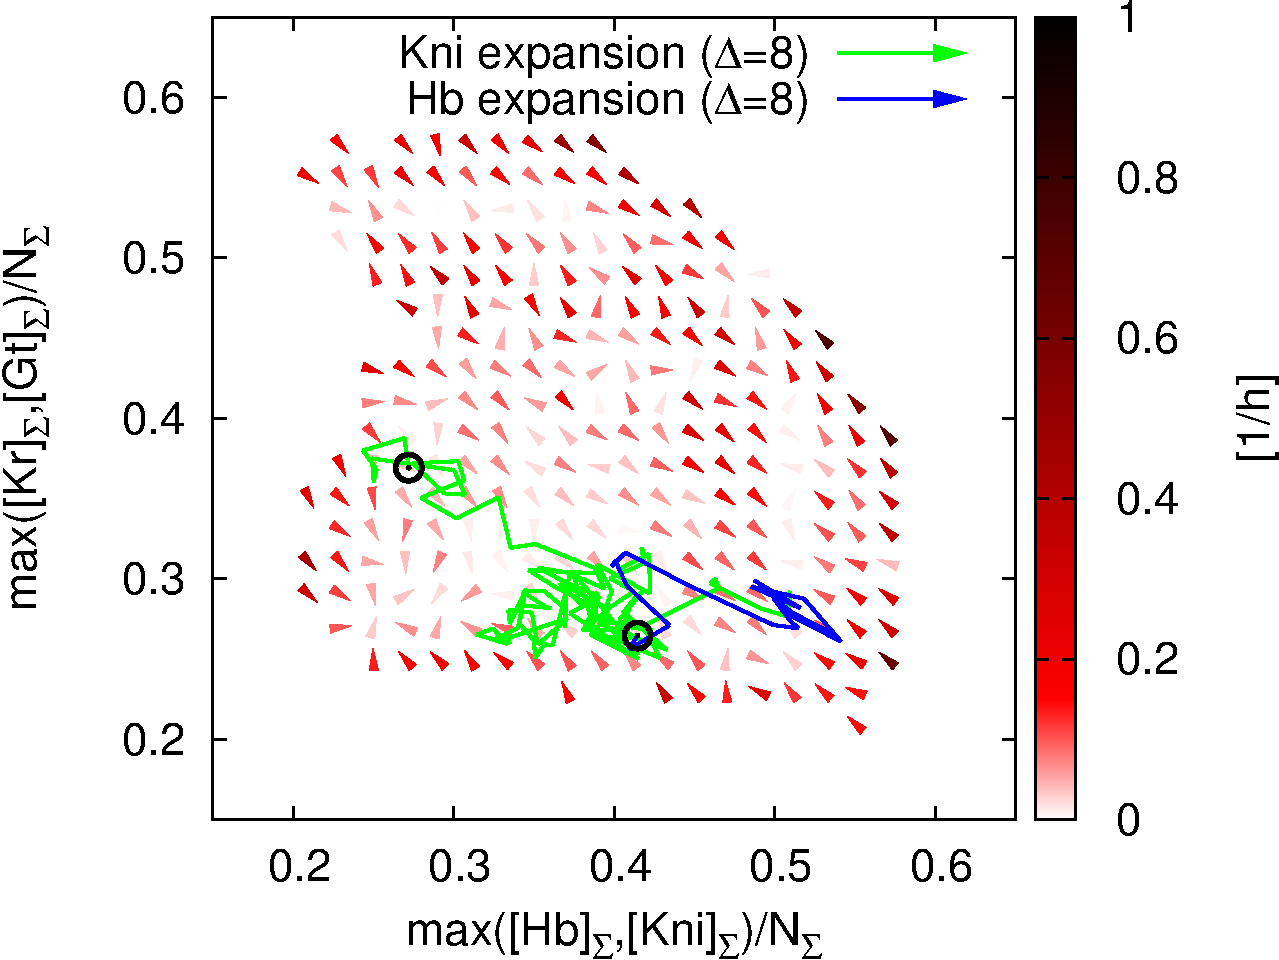
\includegraphics[height=\GGSIVelocityFigureScale]{Figures-SI/FigureVelocitiesUnpinnedOptimum-Relax.pdf}
    \label{Fig-GG-SI-VelocitiesUnpinnedOptimum-Std-Relax}
  }\\
  \subfigure[][]{
    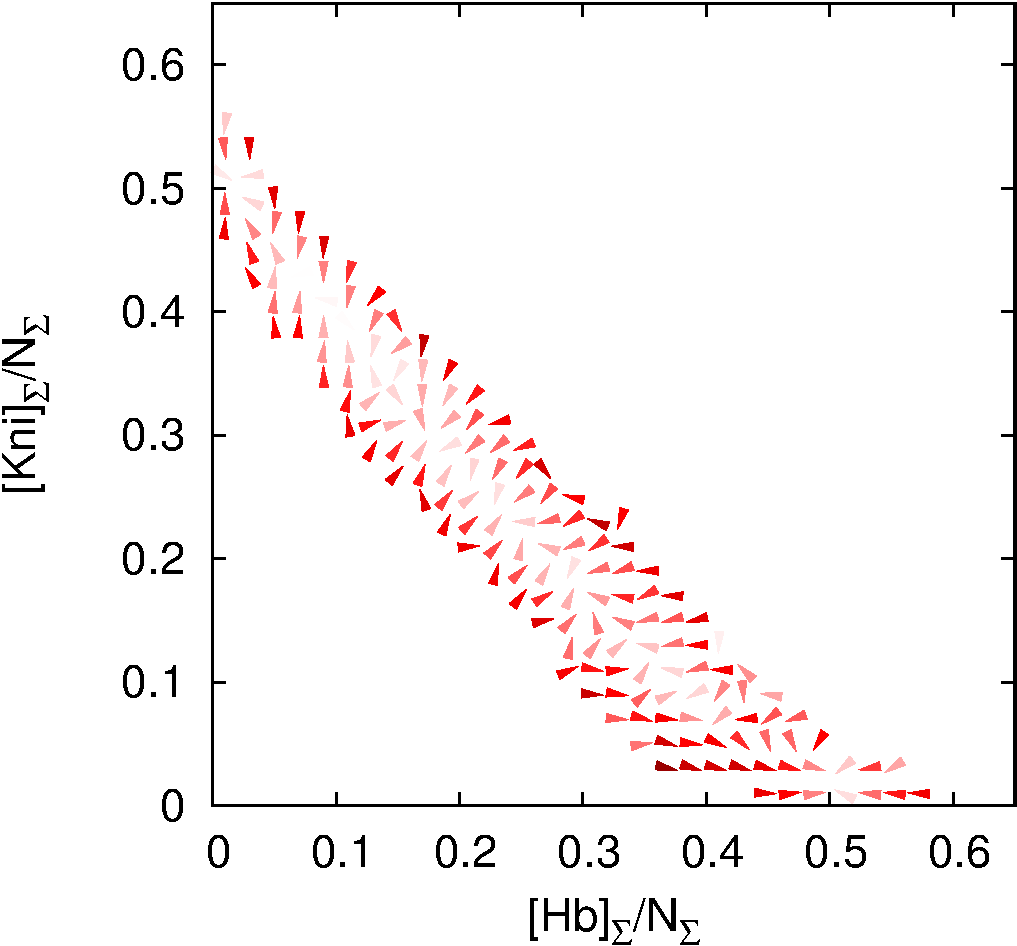
\includegraphics[height=\GGSIVelocityFigureScale]{Figures-SI/FigureVelocitiesUnpinnedOptimumHbKni.pdf}
    \label{Fig-GG-SI-VelocitiesUnpinnedOptimum-HbKni}
  }
  \subfigure[][]{
    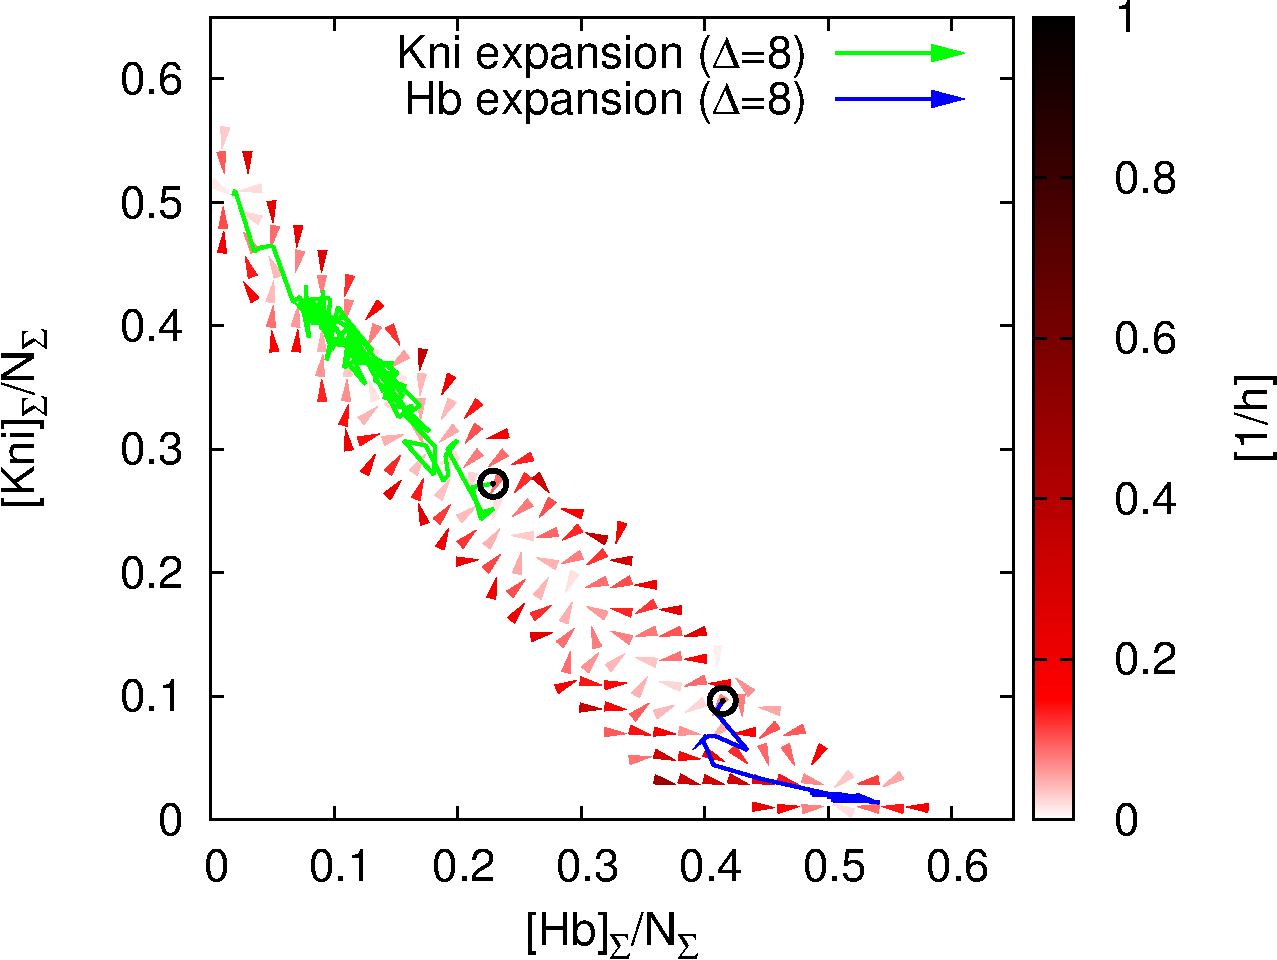
\includegraphics[height=\GGSIVelocityFigureScale]{Figures-SI/FigureVelocitiesUnpinnedOptimumHbKni-Relax.pdf}
    \label{Fig-GG-SI-VelocitiesUnpinnedOptimum-HbKni-Relax}
  }\\
  \subfigure[][]{
    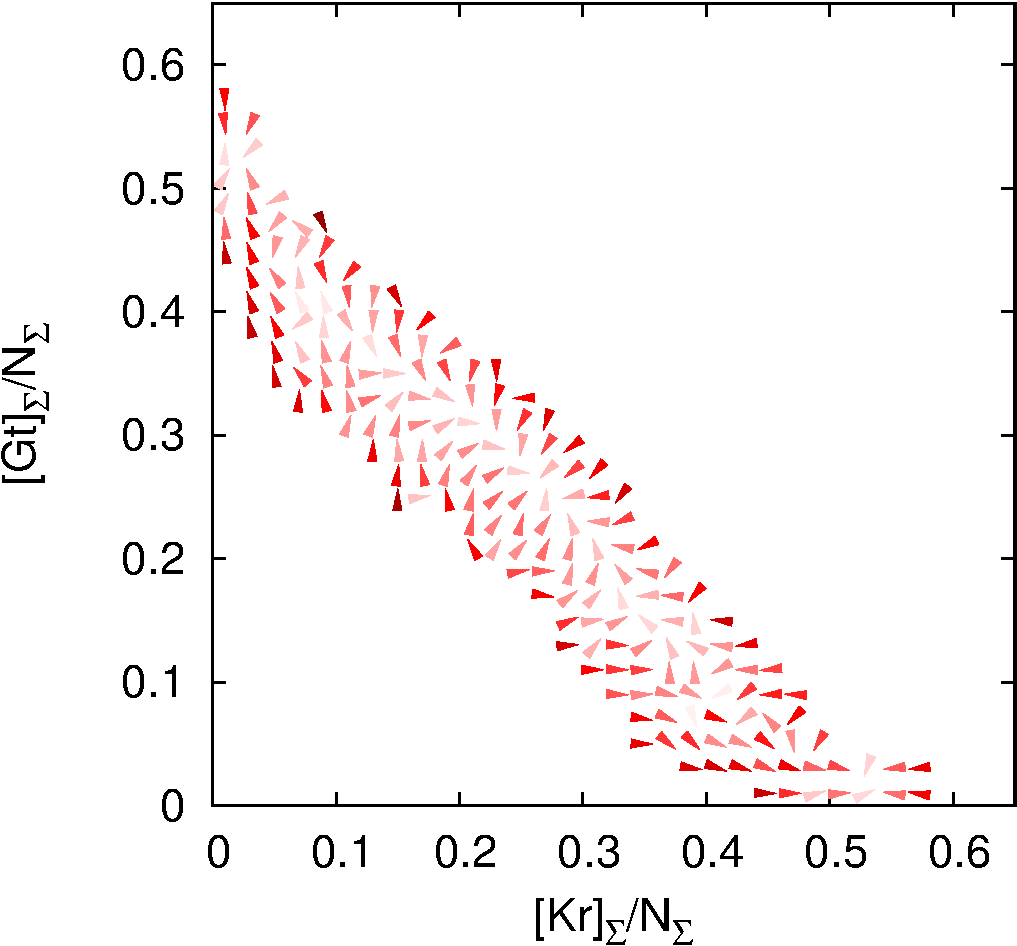
\includegraphics[height=\GGSIVelocityFigureScale]{Figures-SI/FigureVelocitiesUnpinnedOptimumKrGt.pdf}
    \label{Fig-GG-SI-VelocitiesUnpinnedOptimum-KrGt}
  }
  \subfigure[][]{
    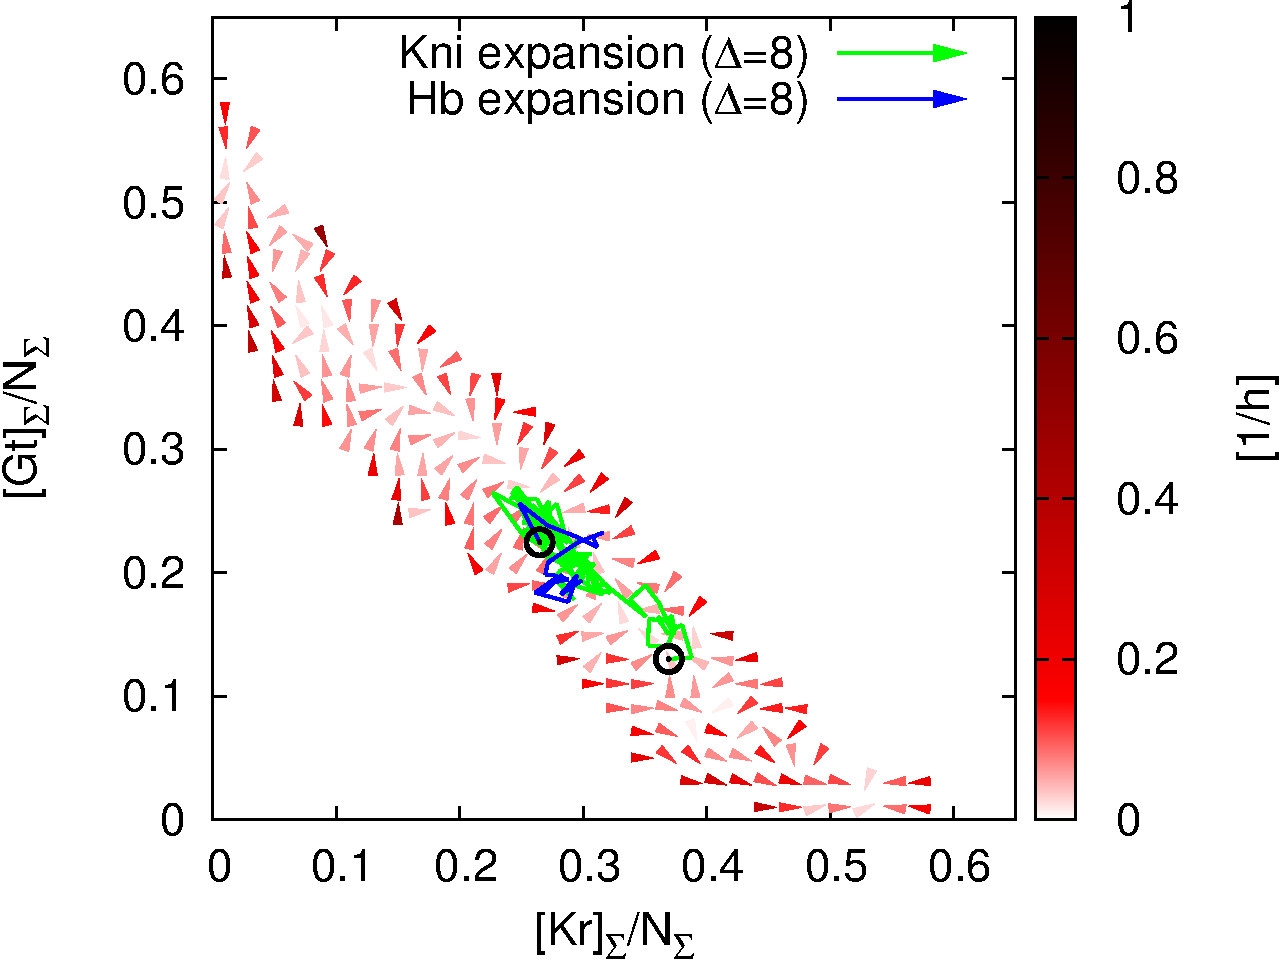
\includegraphics[height=\GGSIVelocityFigureScale]{Figures-SI/FigureVelocitiesUnpinnedOptimumKrGt-Relax.pdf}
    \label{Fig-GG-SI-VelocitiesUnpinnedOptimum-KrGt-Relax}
  }
  \caption{\textbf{Average phase space velocities for the maximally stable system ($\kappa=100$) without pinning.}
    Left plots (A, C, E) show local average phase space velocities, right plots (B, D, F) additionally show 
    example trajectories for the two types of perturbations considered in the restoration experiments.
    Starting points are marked by black bullets.
    %Velocity magnitude is denoted by color on a range from $0$ (white) to $1.0/\mathrm{h}$ (black) with bright red at $0.15/\mathrm{h}$.
    \TODO{Adapt gene names to (A,B,C,D) scheme !!!}
    \label{Fig-GG-SI-VelocitiesUnpinnedOptimum}
    }
\end{figure}

%%%%%%%%%%%%%%%%%
%%% FIGURE S5 %%%
%%%%%%%%%%%%%%%%%
\begin{figure}[H]
  \centering
  \subfigure[][]{
    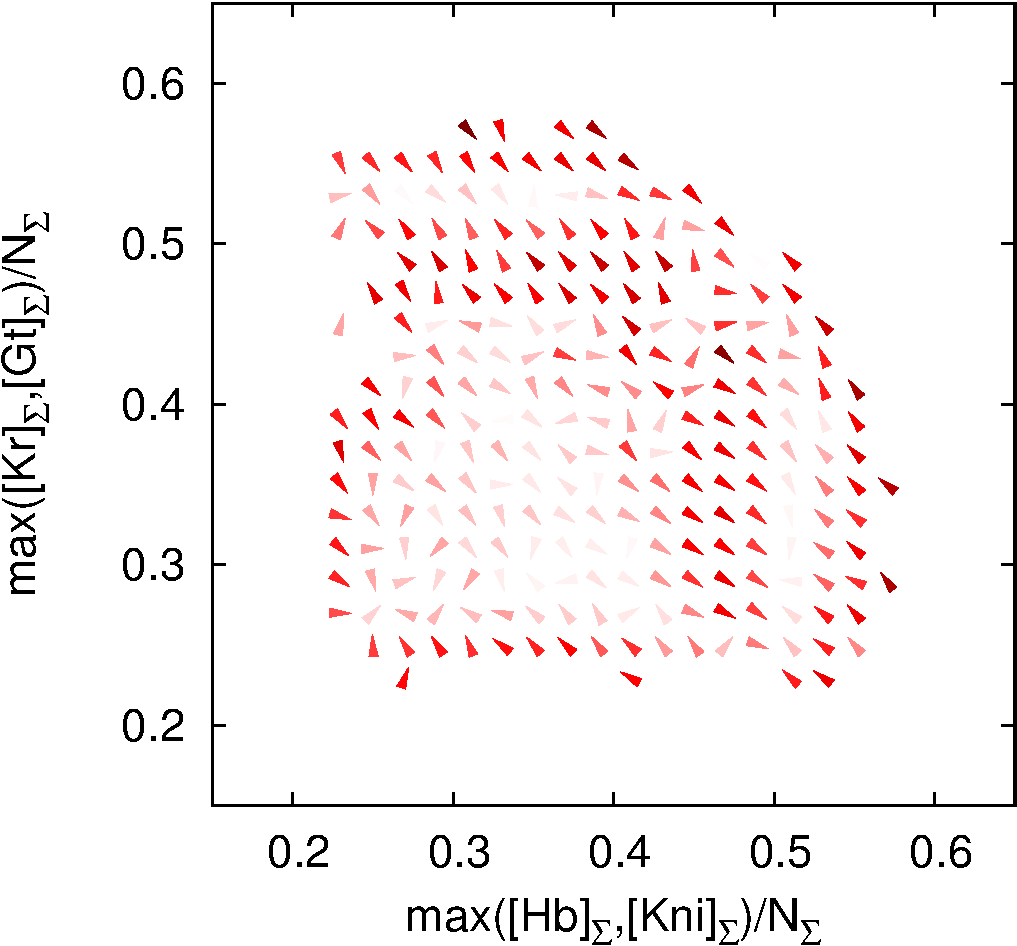
\includegraphics[height=\GGSIVelocityFigureScale]{Figures-SI/FigureVelocitiesUnpinnedKappa1000.pdf}
    \label{Fig-GG-SI-VelocitiesUnpinnedKappa1000-Std}
  }
  \subfigure[][]{
    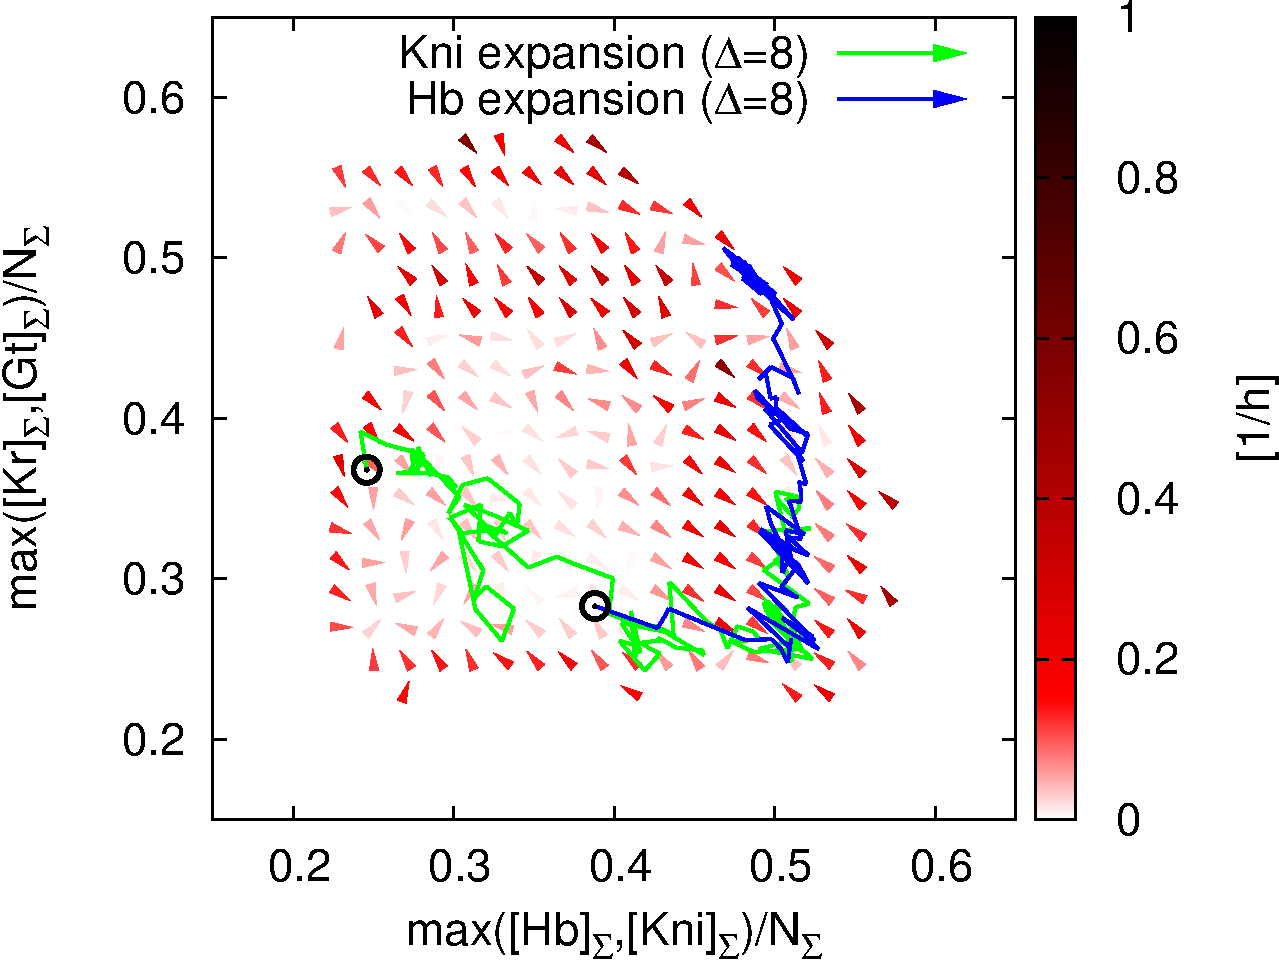
\includegraphics[height=\GGSIVelocityFigureScale]{Figures-SI/FigureVelocitiesUnpinnedKappa1000-Relax.pdf}
    \label{Fig-GG-SI-VelocitiesUnpinnedKappa1000-Std-Relax}
  }\\
  \subfigure[][]{
    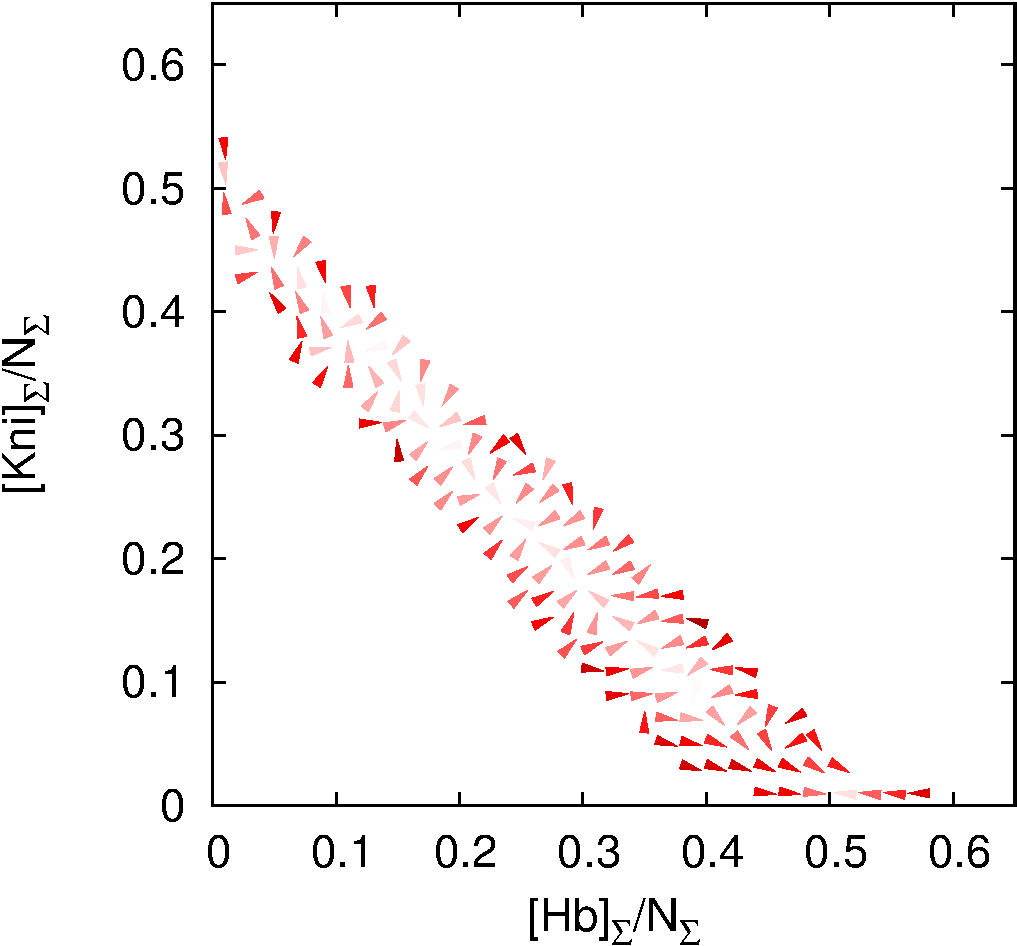
\includegraphics[height=\GGSIVelocityFigureScale]{Figures-SI/FigureVelocitiesUnpinnedKappa1000HbKni.pdf}
    \label{Fig-GG-SI-VelocitiesUnpinnedKappa1000-HbKni}
  }
  \subfigure[][]{
    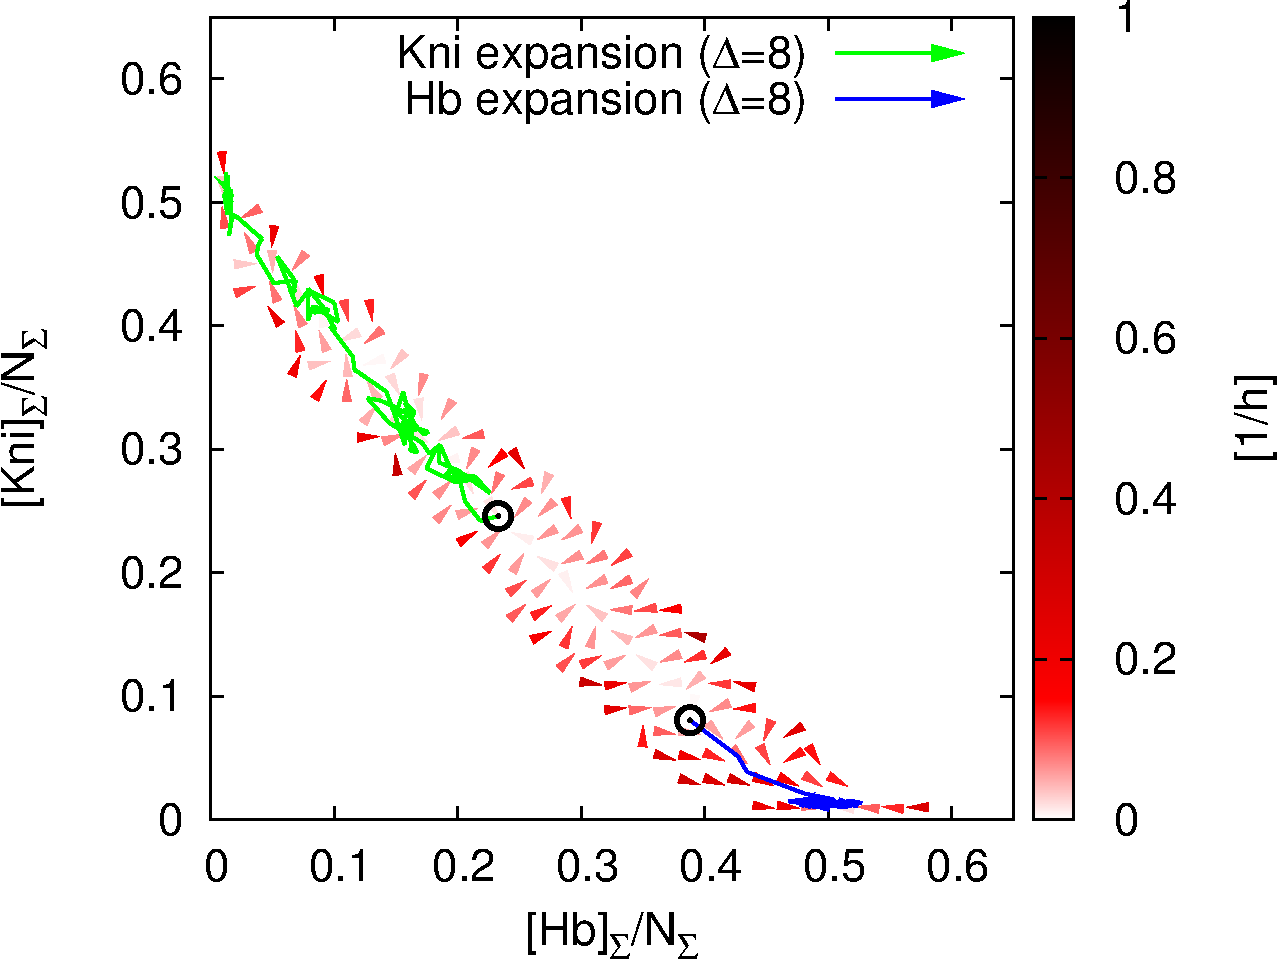
\includegraphics[height=\GGSIVelocityFigureScale]{Figures-SI/FigureVelocitiesUnpinnedKappa1000HbKni-Relax.pdf}
    \label{Fig-GG-SI-VelocitiesUnpinnedKappa1000-HbKni-Relax}
  }\\
  \subfigure[][]{
    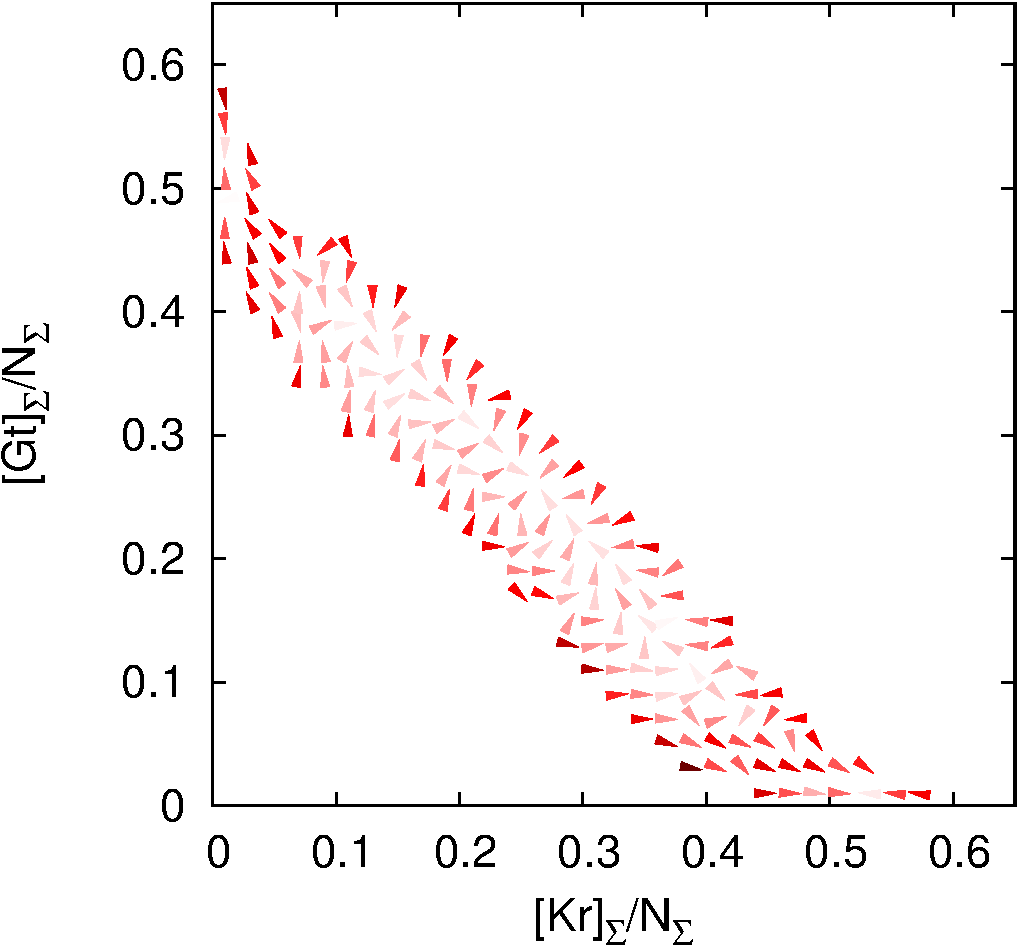
\includegraphics[height=\GGSIVelocityFigureScale]{Figures-SI/FigureVelocitiesUnpinnedKappa1000KrGt.pdf}
    \label{Fig-GG-SI-VelocitiesUnpinnedKappa1000-KrGt}
  }
  \subfigure[][]{
    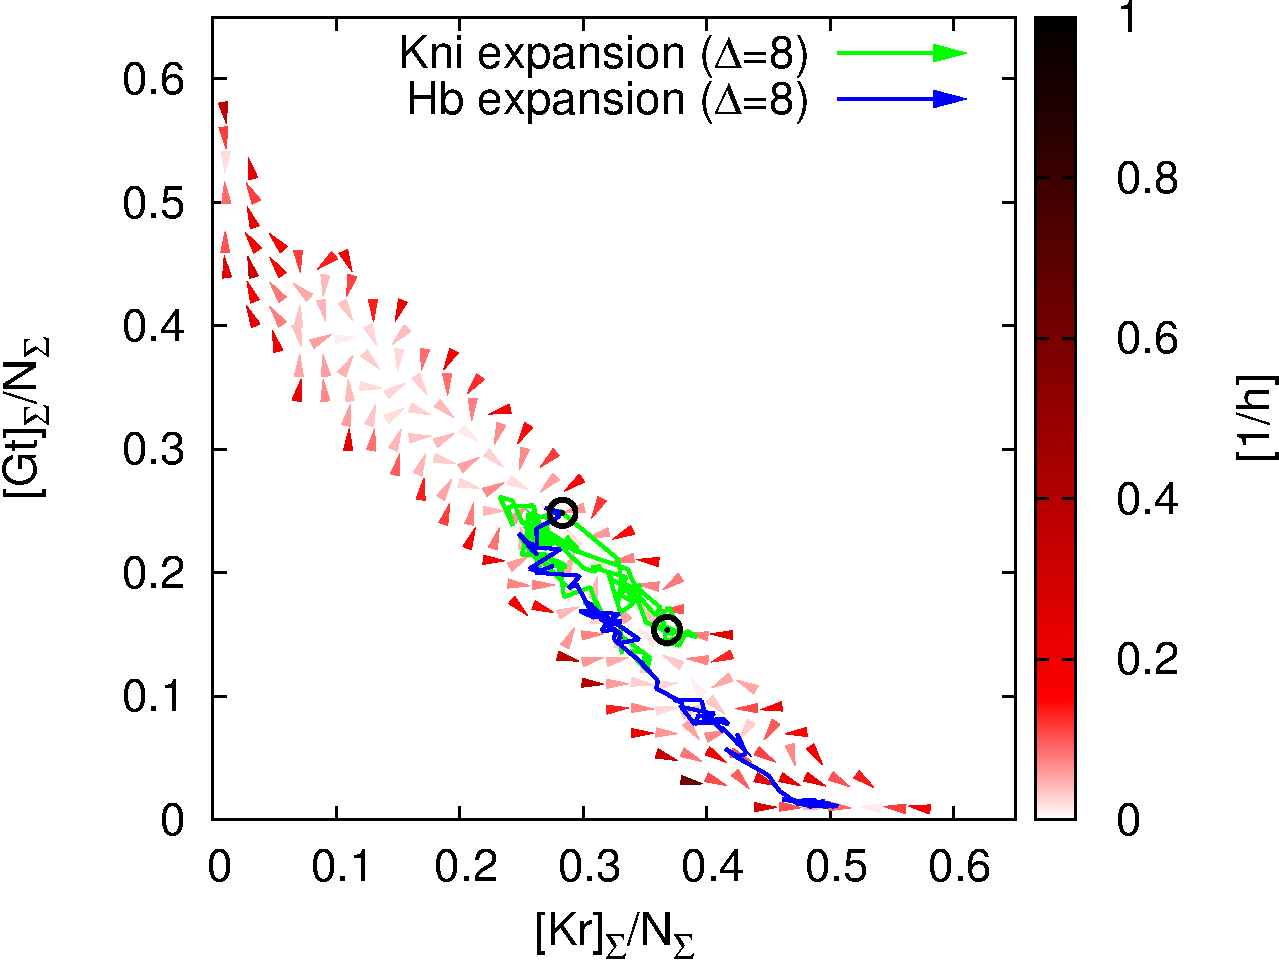
\includegraphics[height=\GGSIVelocityFigureScale]{Figures-SI/FigureVelocitiesUnpinnedKappa1000KrGt-Relax.pdf}
    \label{Fig-GG-SI-VelocitiesUnpinnedKappa1000-KrGt-Relax}
  }
  \caption{\textbf{Average phase space velocities for weaker NN interaction ($\kappa=1000$) in the system without pinning.}
    Left plots (A, C, E) show local average phase space velocities, right plots (B, D, F) additionally show 
    example trajectories for the two types of perturbations considered in the restoration experiments.
    Starting points are marked by black bullets.
    %Velocity magnitude is denoted by color on a range from $0$ (white) to $1.0/\mathrm{h}$ (black) with bright red at $0.15/\mathrm{h}$.
    \TODO{Adapt gene names to (A,B,C,D) scheme !!!}
    \label{Fig-GG-SI-VelocitiesUnpinnedKappa1000}
    }
\end{figure}
\end{comment}


%%%%%%%%%%%%%%%%%
%%% FIGURE S7 %%%
%%%%%%%%%%%%%%%%%
\begin{figure}[ht!]
  \centering
  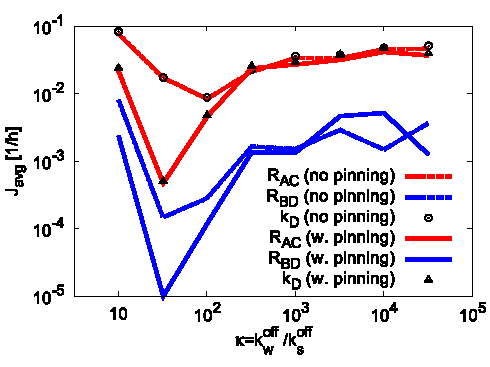
\includegraphics[width=0.8\textwidth]{Figures-SI/FigureFluxes.pdf}
\caption{\textbf{Pinning affects destruction pathways} 
    We plot here the average probability fluxes from the region of stable patterns $R_S$
    into the different remote basins identified in the ($\lambda_{AC},\lambda_{BD}$) phase space
    as a function of the repression strength ratio $\kappa$ for the systems with and without pinning.
    Here the flux is defined as the average increase per time of the total probability in the basin.
    Basin boundaries and flux quantities are described in detail in \MM.
    Shown are the flux into the basin $R^\dagger_{AC}$, corresponding to destruction of either the \GA or \GC domain (red lines),
    the flux into the basin $R^\dagger_{BD}$, in which either the \GB or \GD domain breaks down (blue lines),
    and the total outflux from $R_S$, which equals the pattern destruction rate $k_D$ (black bullets).    
    Solid lines and triangles show the data for the system with pinning, dashed lines and circles the values for
    the system without pinning.
    Clearly, in both with and without pinning and for all $\kappa$ considered here, $R^\dagger_{AC}$ is the dominant
    fraction of the flux, reflecting that the dominant pathway to destruction is the one that starts with the 
    disappearance of either the \GA or \GC domain.
    Pinning of \GA expression at the system boundaries leads to a pronounced reduction of the flux through this
    pathway for $\kappa=10 - 100$.
  \label{Fig-Fluxes}
}
\end{figure}

\clearpage

%%%%%%%%%%%%%%%%%
%%% FIGURE S8 %%%
%%%%%%%%%%%%%%%%%
\begin{figure}[ht]
  \centering
  \subfigure{
      \label{Fig-FluxesACPinned}
      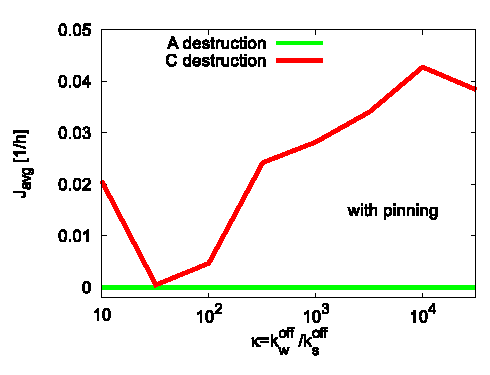
\includegraphics[width=0.66\textwidth]{Figures-SI/FigureFluxesACPinned.pdf}
  }
  \subfigure{
      \label{Fig-FluxesACUnpinned}
      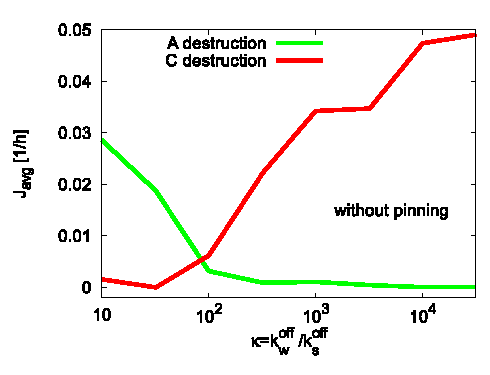
\includegraphics[width=0.66\textwidth]{Figures-SI/FigureFluxesACUnpinned.pdf}
  }
\caption{\textbf{Pinning shifts the destruction flux balance in the dominant (\GA-\GC) destruction pathway}
    The figure shows the contributions of the \GA-destruction and \GC-destruction pathways to the outflux from $R_S$
     as a function of the repression strength ratio $\kappa$ for the systems with \mysubref{Fig-FluxesACPinned}
    and without \mysubref{Fig-FluxesACUnpinned} pinning.
    See \MM for the definitions of basin boundaries and details of flux calculation.	  	  
    Without pinning and for strong NN repression, the preferred pathway to
    destruction is the one in which the \GA domains are destroyed first, while for weaker coupling (large $\kappa$)
    destruction begins via annihilation of the \GC domain.
    Interestingly, in both cases the flux through the \GC-destruction pathway is minimal at $\kappa\simeq31.6$.
    Pinning forbids destruction via the \GA pathway and thus dramatically reduces the overall destruction flux
    for low $\kappa$, giving rise to the enhanced stability optimum at $\kappa\simeq31.6$.
  \label{Fig-FluxesDominantPathway}
}
\end{figure}



\section{Pinning alters the proportion of destruction pathways}

Both with and without pinning of \GA expression at the system boundaries, pattern 
stability is maximal at an optimal strength of NN repression.
Stability times, however, are significantly higher in the system with pinning.
In order to understand whether this is simply due to the fact that pinning prohibits destruction of the \GA domains or 
due to other pinning-induced effects, we compared the different pathways to destruction by computing 
probability fluxes through distinct reaction pathways (see \MM for details).
The different reaction pathways are defined by the order in which gap gene domains are destroyed.
In our system there are two major pathways: the \GA-\GC destruction pathway (either the \GA or the \GC domain vanishes first) 
and the \GB-\GD destruction pathway (either the \GB or \GD domain vanishes first).
The phase space histograms in Figure~3 of the main text demonstrate that simultaneous destruction of two domains,
corresponding to trajectories that progress diagonally in ($\lambda_{AC},\lambda_{BD}$) space, is highly improbable.
We find that, while in general the \GA-\GC destruction pathway prevails, 
the fact that the \GA-destruction pathway is dominant for $\kappa\leq100$ in the system without pinning 
accounts for the strong enhancement of pattern stability due to pinning.

In Figure \ref{Fig-Fluxes} we plot for different repression strength ratios $\kappa$
the magnitude of average fluxes from the region of intact patterns $R_S$ in the ($\lambda_{AC},\lambda_{BD}$) space 
into the respective neighboring regions that correspond to states in which one expression domain vanished.
The figure reveals that for all $\kappa$ the flux through the \GA-\GC destruction pathway is approximately 
ten times higher than the flux through the \GB-\GD pathway, for systems both with and without pinning.
The figure also shows that pinning indeed reduces the flux through the dominant, 
i.e. \GA-\GC, pathway, most significantly for $\kappa\simeq 10-100$, i.e. around the optimal value $\kappa_{opt}$. 
This gives rise to the pronounced stability enhancement.
The simultaneous reduction of the flux through the \GB-\GD pathway is not relevant for overall stability.
% however this is negligible given the clear predominance of the other pathway.

We analysed further the detailed composition of fluxes through the dominant (\GA-\GC) pathway 
by computing the average flux into the regions of destroyed states in $([\GA]_{tot}/N_{tot},[\GC]_{tot}/N_{tot})$ space, see Fig.~\ref{Fig-FluxesDominantPathway}.
% The results are shown in Figure \ref{Fig-FluxesDominantPathway} for the systems with (\subref{Fig-FluxesHbKniPinned})
% and without (\subref{Fig-FluxesHbKniUnpinned}) pinning.
As expected, in the systems with pinning the entire flux through the dominant pathway goes into the \GC-destroyed state.
Interestingly, this is also the case for the weakly coupled systems without pinning.
Here the flux into the \GA-destroyed state is clearly dominant over the flux into the \GC-destroyed state for strong NN interaction.
This explains why pinning, which prohibits exit through the \GB-destruction pathway, increases stability in the $\kappa \lesssim 100$ regime.
While the flux through the \GC-destruction pathway is minimal at $\kappa=31.6$ with or without pinning,
in the system without pinning the accessibility of \GA destruction shifts the minimum of the combined flux through both pathways
towards $\kappa=100$, see Fig.~\ref{Fig-Fluxes}.

\FloatBarrier

\begin{comment}

\section{Stability analysis of a mutually repressing four gene system}
\label{Sec-SI-StabilityAnalysis}
In order to elucidate the reason for the stabilization of an interface of two strongly antagonistic 
gene expression domains in the presence of further, weak interaction partners we conducted a linear
stability analysis on a deterministic ODE system in steady state, which mimics the situation in a typical
interface nucleus in our full-scale system.
To model the particular situation in such a nucleus more accurately we introduce flux terms into the ODEs,
which--in an approximative fashion--take into account the diffusive exchange of particles with neighboring nuclei.

We analysed the following set of 8 equations that describe the production, degradation
and (de)dimerization of four mutually repressing genetic species A, B, C and D:
\begingroup
\addtolength{\jot}{2em} % nicer spacing of equations
\begin{align}
\partial_t A_1	&= \frac{\beta}{(1+B_2/K_s)(1+C_2/K_w)(1+D_2/K_w)} - \mu_M A_1 - \kDon A_1^2 + \kDoff A_2 = 0	\nn\\
\partial_t A_2	&= \kDon A^2 - (\kDoff + \mu_D) A_2 + j_{A_2}= 0						\nn\\
\partial_t B_1	&= \frac{\beta}{(1+A_2/K_s)(1+C_2/K_w)(1+D_2/K_w)} - \mu_M B_1 - \kDon B_1^2 + \kDoff B_2 = 0	\nn\\
\partial_t B_2	&= \kDon B^2 - (\kDoff + \mu_D) B_2 + j_{B_2}= 0						\nn\\
\partial_t C_1	&= \frac{\beta}{(1+D_2/K_s)(1+A_2/K_w)(1+B_2/K_w)} - \mu_M C_1 - \kDon C_1^2 + \kDoff C_2 = 0	\nn\\
\partial_t C_2	&= \kDon C^2 - (\kDoff + \mu_D) C_2 + j_{C_2} = 0						\nn\\
\partial_t D_1	&= \frac{\beta}{(1+C_2/K_s)(1+A_2/K_w)(1+B_2/K_w)} - \mu_M D_1 - \kDon D_1^2 + \kDoff D_2 = 0	\nn\\
\partial_t D_2	&= \kDon D^2 - (\kDoff + \mu_D) D_2 + j_{D_2} = 0
\end{align}
\endgroup

Here capital letters $X_1$ denote monomer numbers, while capital letters with index $X_2$ describe
dimer numbers; the total copy number is defined as $X=X_1+2X_2$.
The (monomer) production rate $\beta$, the monomeric and dimeric degradation rates $\mu_M$ and $\mu_D$ 
and the dimerization forward and backward rates $\kDon$ and $\kDoff$ are equal for all four species, in
correspondence to our full-scale model.
The four genes thus have identical properties, except for the strength by which a gene is repressed by the
other genes, which is tuned via two repression threshold parameters (dissociation constants) $K_s$ and $K_w$.
Here $K_s$ stands for strong, $K_w$ for weaker mutual repression, i.e. $K_s < K_w$.
The ratio $\kappa = K_w / K_s$ corresponds to the repression strength ratio parameter $\kappa$ in the main text.
For each gene X the term $j_{X_2}$ represents an effective dimeric flux into or out of the considered nucleus
due to dimer exchange with neighboring nuclei.
To facilitate calculations we assume that in steady state these fluxes are constant;
flux magnitudes are estimated from our spatially resolved simulations, as explained further below.
As a further simplification we neglect the monomeric fluxes. This is justified by the fact that in our model
the monomer degradation rate is one order of magnitude higher than the dimer degradation rate, translating into
a significantly shorter diffusion length for the monomers.

The analysis was performed by numerically solving the above steady-state equations for fixed point solutions.
Stability was determined by calculating the eigenvalues of the corresponding Jacobian at the fixed point to
discriminate between stable (all eigenvalues with negative real part), 
unstable (at least one eigenvalue with positive real part) and oscillatory solutions.
All parameter values were chosen in correspondence to the full scale model (see Table \ref{Tab-GG-SI-Parameters}),
while $\kappa$ was varied via $K_w$ as in the simulations.

We first analysed the system without dimeric fluxes, i.e. $j_{X_2}=0$ for ${\rm X}\in \lbrace {\rm A, B, C, D} \rbrace$.
Figure \ref{Fig-GG-SI-StabAnalysisNoFlux-3D} shows 3D plots of two different 2D projections of the
four-dimensional fixed point solutions for the total copy numbers ${\rm (A,B,C,D)}$ as a function of $\kappa$,
the ratio between weak and strong repression threshold.
Here we employ the fact that, due to the repeating interaction symmetry, the change of 4D attractor locations with $\kappa$ 
can be understood by looking at the change of attractor locations in the 2D spaces spanned by the components 
of two strongly and two weakly repressing species, respectively.
In Figure \ref{Fig-GG-SI-StabAnalysis-2D}A-D we additionally plot 1D projections of the four single components, 
which, in this case, are identical.
The plots reveal two principal fixed point regimes: A ``monostable regime'' in which only one of four genes can attain high
expression levels for low $\kappa$ and a ``coexistence regime'' of two bistable pairs in which
each state of one bistable pair can coexist with each state of the other bistable pair.
The two regimes are separated by a bifurcation that occurs around $\kappa \simeq \kappaBif$.
Note that when A is high on the weak partners branch (blue) in Fig. \ref{Fig-GG-SI-StabAnalysisNoFlux-3D}
(and its weak partner C therefore low) within the monostable regime ($\kappa \lesssim \kappaBif$), the corresponding points 
on the strong partners branch (red) are the ones in the low-expression regime close to zero, and vice versa.
Interestingly, at $\kappa=1$ we find an additional stable fixed point at which all four genes have very low 
expression levels ($\rm A = B = C = D \simeq 1$), meaning that when all genes suppress each other equally strongly one
possible outcome is that none of them can reach significant expresssion levels.
Taken together this demostrates that for $\kappa \lesssim \kappaBif$ solutions in which two genes are expressed 
at significant levels are unstable.
Given a certain minimal domain size required in a system with finite repressor diffusion length
this implies instability of the whole partly overlapping five-stripe pattern and thus provides an explanation
for fast pattern destruction in the strong coupling regime.

As a second step we repeated the stability analysis with nonzero dimer fluxes,
in order to mimic the situation in a nucleus at the \Hb-\Kni expression boundaries interface.
To this end we imposed a dimer influx for the two strong antagonists A and B
and a dimer outflux for C, which is a weak partner of both A and B,
with flux magnitudes approximately equal to average fluxes estimated on the base
of time- and circumference-averaged stationary profiles from simulations of the 
system with pinning at optimal $\kappa$.
These fluxes were estimated by first finding the nuclear row $N_i$ at the $\Hb-\Kni$ interface,
computing the stationary copy number gradients $\Delta N_{-}$ and $\Delta N_{+}$ with respect to the 
preceding and subsequent rows via finite differences and then multiplying their difference
with the diffusive hopping rate, i.e.:
\begin{align}
j_{est} &\equiv (\Delta N_{+} - \Delta N_{-}) \frac{4D}{l^2}
\end{align}
where $l$ is the (constant) distance between nuclei.

Figure \ref{Fig-GG-SI-StabAnalysis-2D}E-H demonstrates that imposing dimeric fluxes as described
has a dramatic effect on the fixed point solutions of the system.
Here we could not find any physically meaningful stable fixed points for $\kappa \lesssim 12$.
For higher values of $\kappa$ we find that there is only one stable solution:
Maybe contrary to expectation, an influx of A and B dimers
results in a significant reduction of the expression levels of these genes, while gene C,
in spite of the assumed outflux, reaches high expression levels.
Consequently, production of D is strongly suppressed.
The total copy numbers at the fixed points are in good agreement with 
typical copy numbers at the interface between strongly repressing gene domains in our simulations.

\clearpage
In summary, our analysis predicts that when all genes repress each other with close to equal
strength ($\kappa \lesssim \kappaBif$) patterns with overlapping gap gene domains are intrinsically unstable.
It further indicates that a small net influx of two strongly repressing partners A and B and outflux of
one of their weak interaction partners C may result in
the counterintuitive effect that the expression level of A and B will be significantly reduced
while C is stabilized at higher levels.

\clearpage


%%%%%%%%%%%%%%%%%
%%% FIGURE S7 %%%
%%%%%%%%%%%%%%%%%
\begin{figure}[H]
  \centering
  \subfigure[][]{
    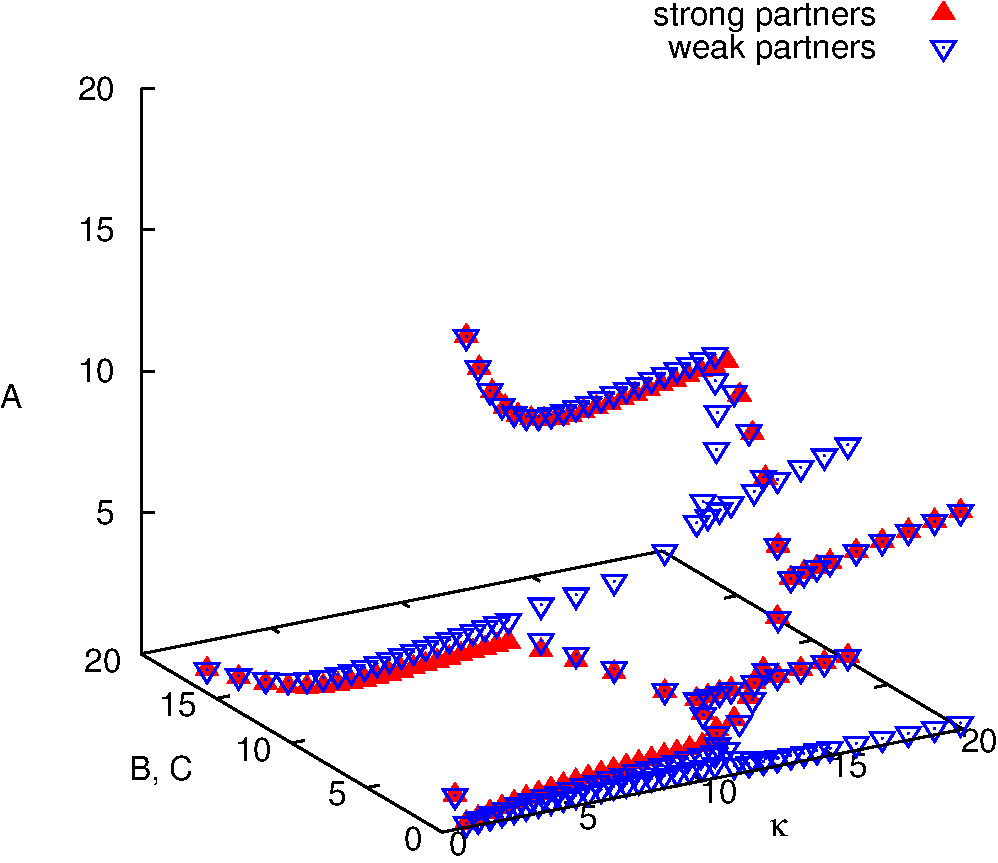
\includegraphics[width=0.45\textwidth]{Figures-SI/FigureFixpointsNoFlux-3D-1.pdf}
    \label{Fig-GG-SI-StabAnalysisNoFlux-3D-1}
  }\hfill
  \subfigure[][]{
    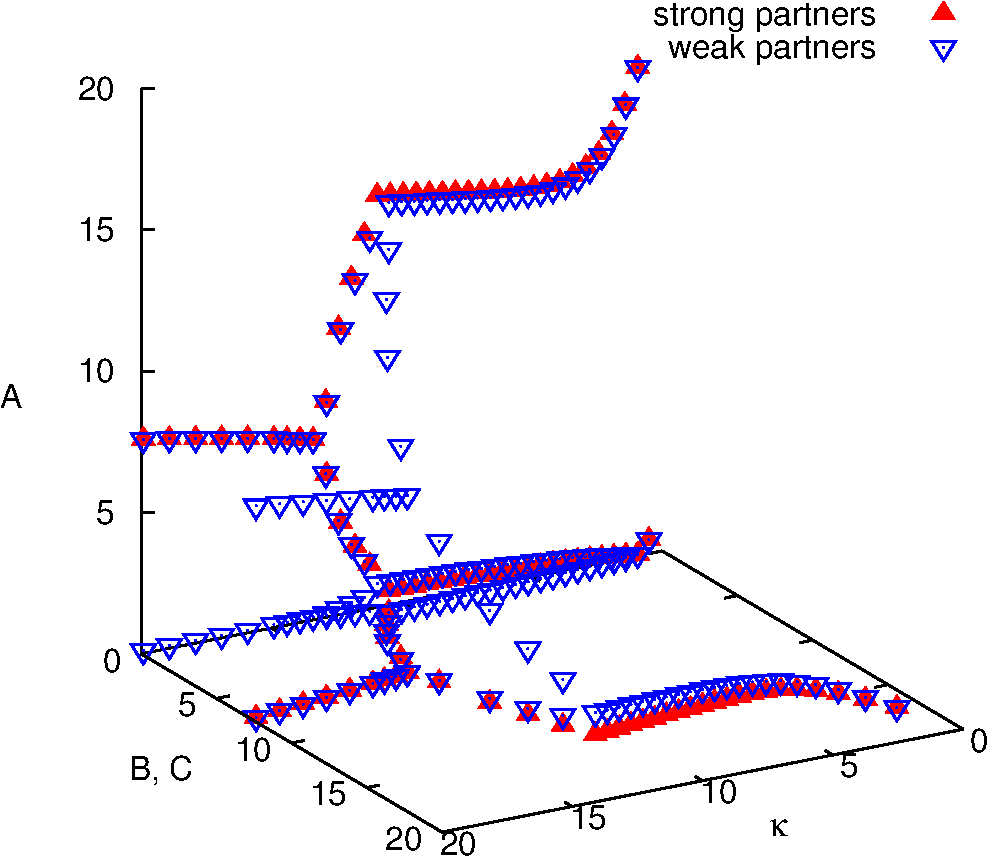
\includegraphics[width=0.45\textwidth]{Figures-SI/FigureFixpointsNoFlux-3D-2.pdf}
    \label{Fig-GG-SI-StabAnalysisNoFlux-3D-2}
  }\\
  \subfigure[][]{
    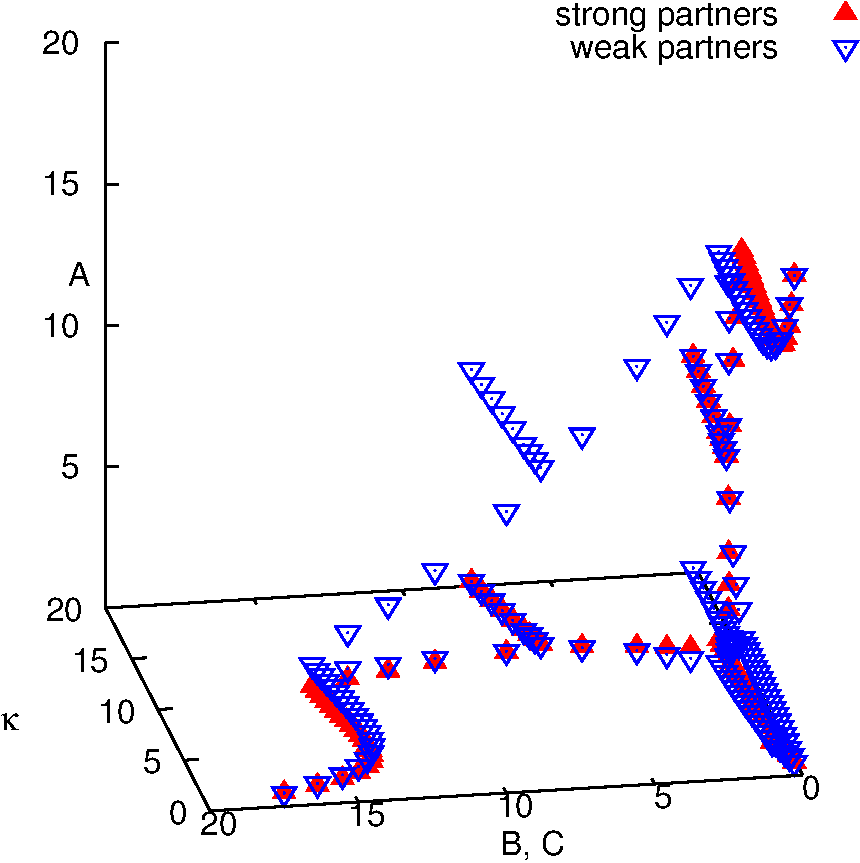
\includegraphics[width=0.45\textwidth]{Figures-SI/FigureFixpointsNoFlux-3D-3.pdf}
    \label{Fig-GG-SI-StabAnalysisNoFlux-3D-3}
  }\hfill
  \subfigure[][]{
    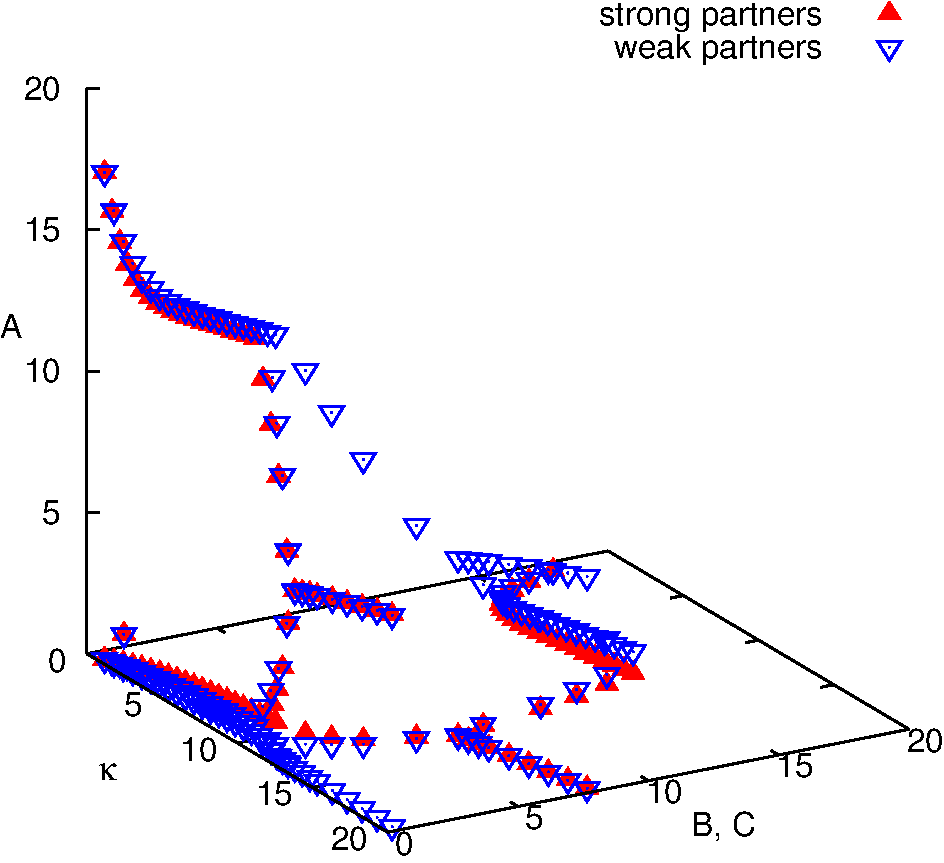
\includegraphics[width=0.45\textwidth]{Figures-SI/FigureFixpointsNoFlux-3D-4.pdf}
    \label{Fig-GG-SI-StabAnalysisNoFlux-3D-4}
  }
  \caption{\textbf{Steady state stability analysis with zero dimer fluxes.}
    Shown are 2D projections of stable fixed point solutions
    ${\rm (A,B,C,D)}$ for the total copy numbers (monomers + dimers)
    of the considered mutually repressing four-gene system as a function of $\kappa$,
    the ratio between weak and strong repression thresholds.   
    Each plot contains data for two different projections: ${\rm (A,B)}$, i.e.
    strong interaction partners (red triangles), and ${\rm (A,C)}$, i.e. weak interaction partners (blue triangles).
    Note that for the analysed system projections ${\rm (A,B)}$ and $(C,D)$
    and projections ${\rm (A,C)}$, ${\rm (A,D)}$, ${\rm (B,C)}$ and ${\rm (B,D)}$
    are identical for symmetry reasons.
    Panels A-D display the same data in different viewing perspective.
  \label{Fig-GG-SI-StabAnalysisNoFlux-3D}
}
\end{figure}



\newcommand{\GGSIFixpointsPlotScale}{0.35\textwidth}
\newcommand{\GGSIFixpointsPlotHspace}{\hspace{22pt}}
\renewcommand{\subfigcapskip}{-12pt}
\renewcommand{\subfigcapmargin}{-22pt}
%%%%%%%%%%%%%%%%%
%%% FIGURE S8 %%%
%%%%%%%%%%%%%%%%%
\begin{figure}[H]
  \centering
  \GGSIFixpointsPlotHspace
  \subfigure[][]{
    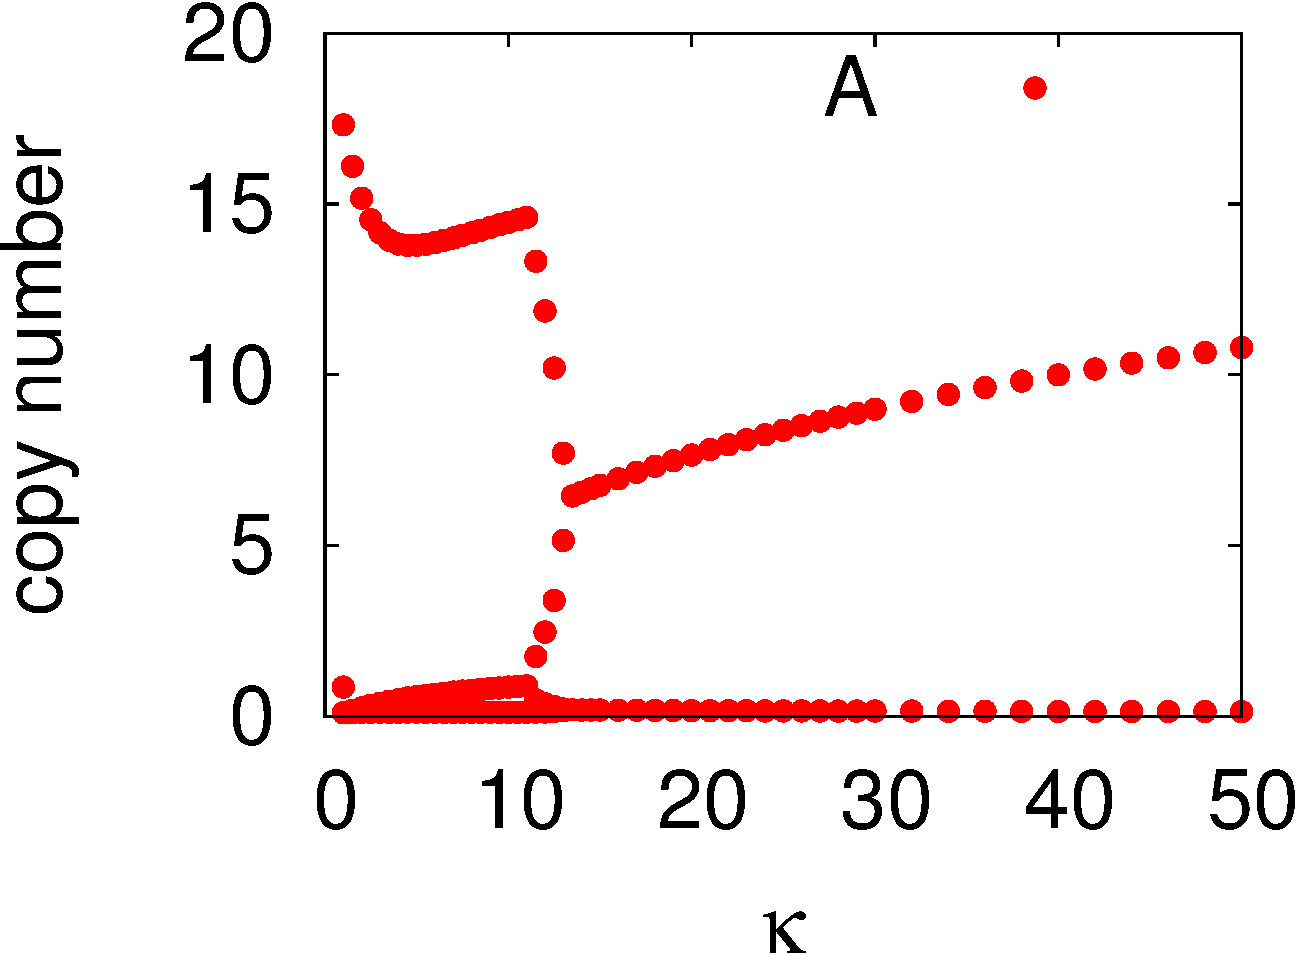
\includegraphics[width=\GGSIFixpointsPlotScale]{Figures-SI/FigureFixpointsNoFlux-A.pdf}
    \label{Fig-GG-SI-StabAnalysisNoFlux-2D-A}
  }
  \GGSIFixpointsPlotHspace\GGSIFixpointsPlotHspace
  \subfigure[][]{
    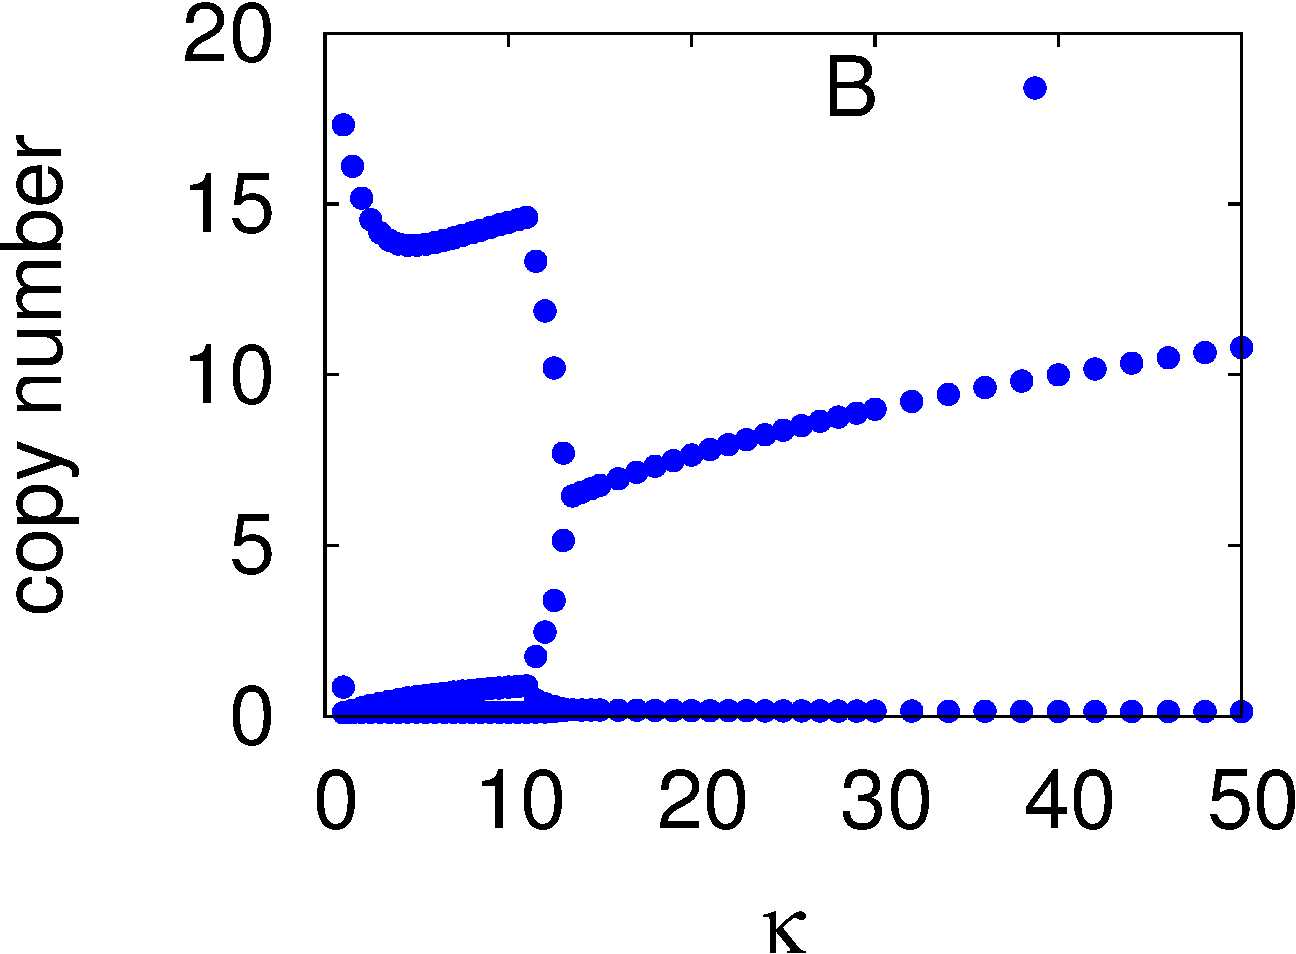
\includegraphics[width=\GGSIFixpointsPlotScale]{Figures-SI/FigureFixpointsNoFlux-B.pdf}
    \label{Fig-GG-SI-StabAnalysisNoFlux-2D-B}
  }\\
  \GGSIFixpointsPlotHspace
  \subfigure[][]{
    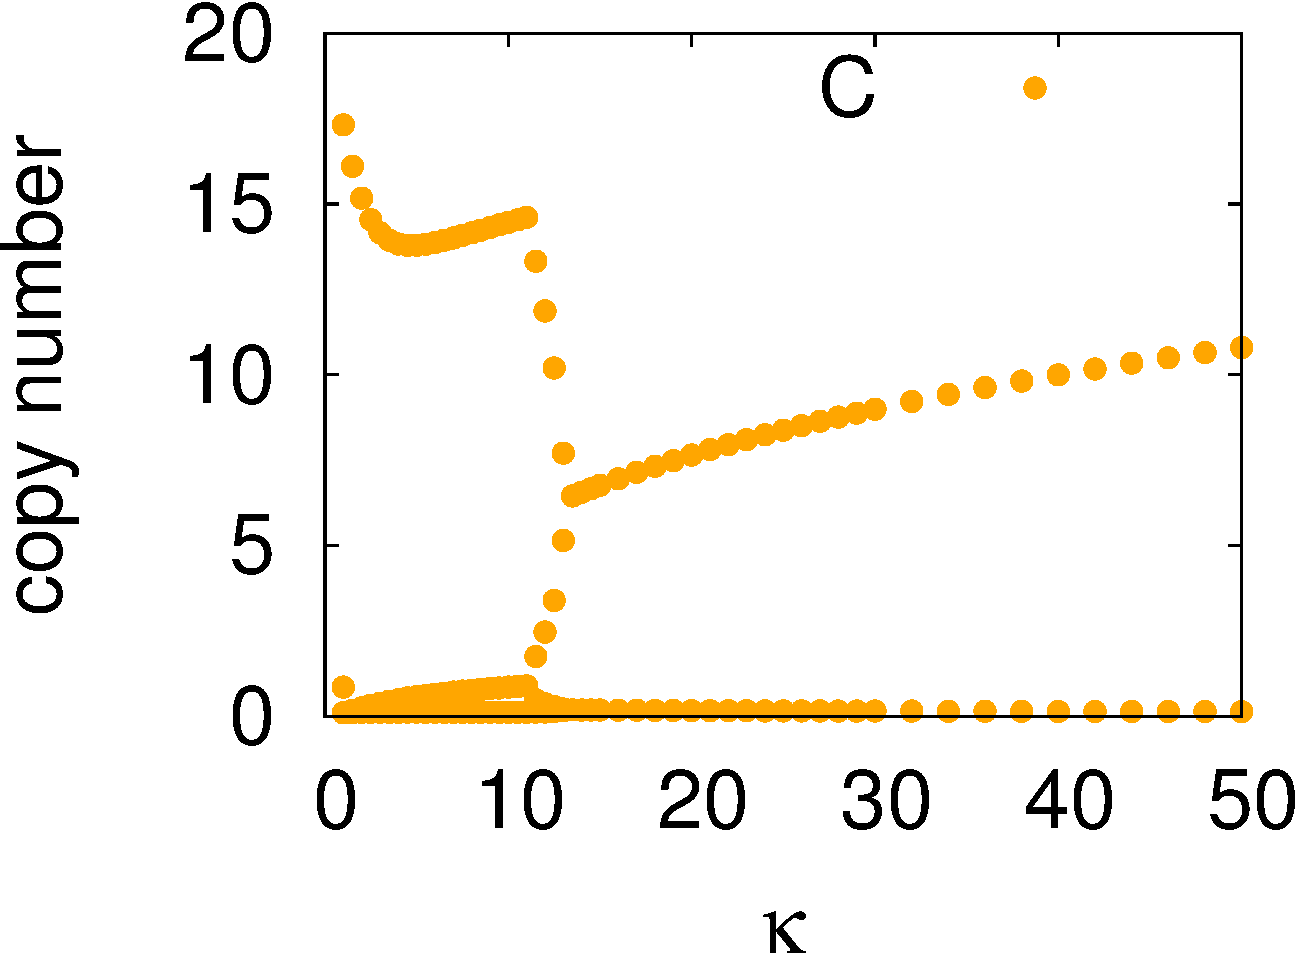
\includegraphics[width=\GGSIFixpointsPlotScale]{Figures-SI/FigureFixpointsNoFlux-C.pdf}
    \label{Fig-GG-SI-StabAnalysisNoFlux-2D-C}
  }
  \GGSIFixpointsPlotHspace\GGSIFixpointsPlotHspace
  \subfigure[][]{
    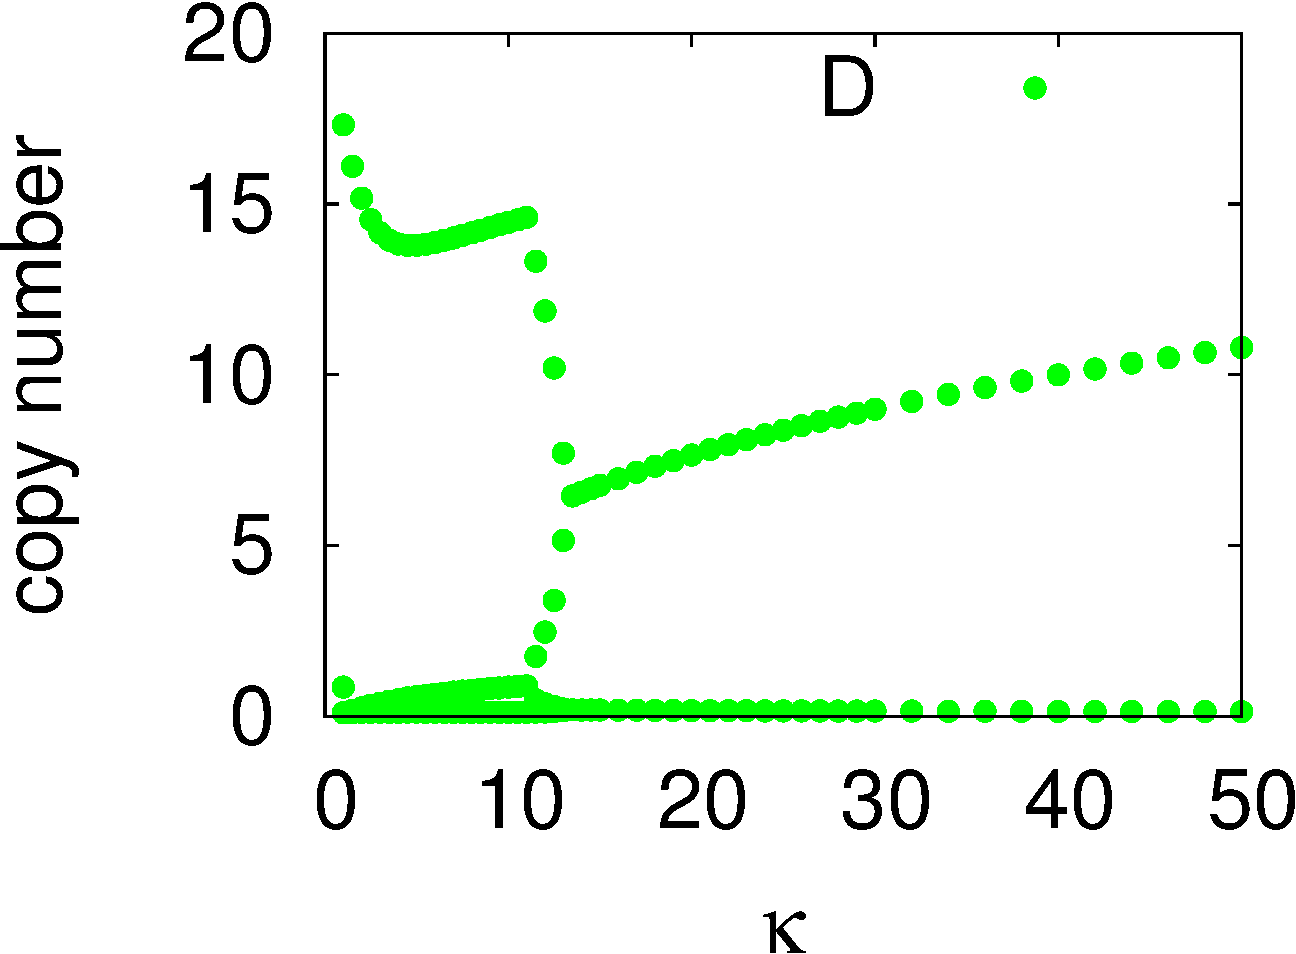
\includegraphics[width=\GGSIFixpointsPlotScale]{Figures-SI/FigureFixpointsNoFlux-D.pdf}
    \label{Fig-GG-SI-StabAnalysisNoFlux-2D-D}
  }\\
  \GGSIFixpointsPlotHspace
  \subfigure[][]{
    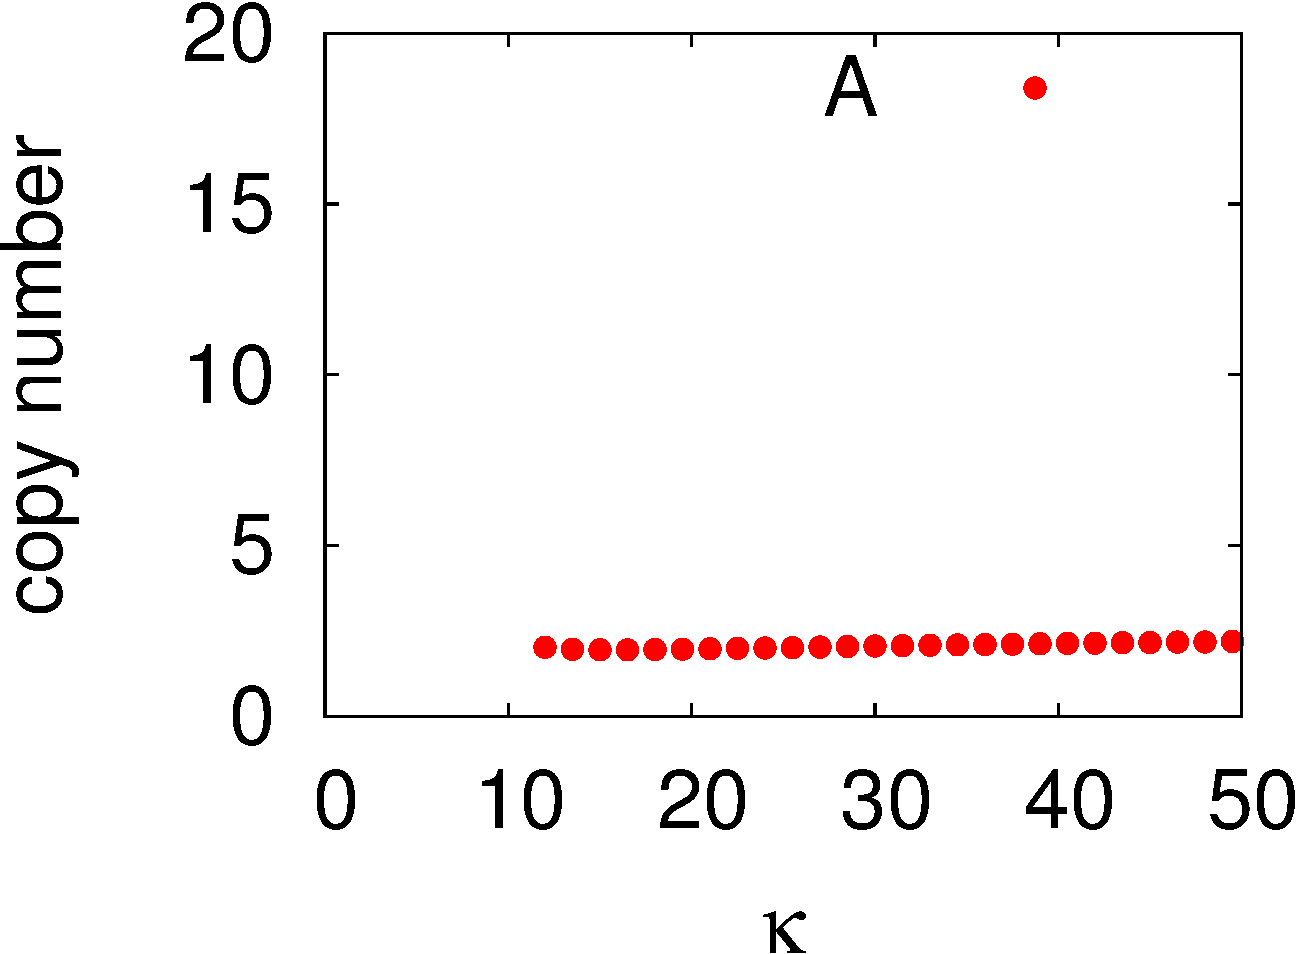
\includegraphics[width=\GGSIFixpointsPlotScale]{Figures-SI/FigureFixpointsWithFlux-A.pdf}
    \label{Fig-GG-SI-StabAnalysisWithFlux-2D-A}
  }
  \GGSIFixpointsPlotHspace\GGSIFixpointsPlotHspace
  \subfigure[][]{
    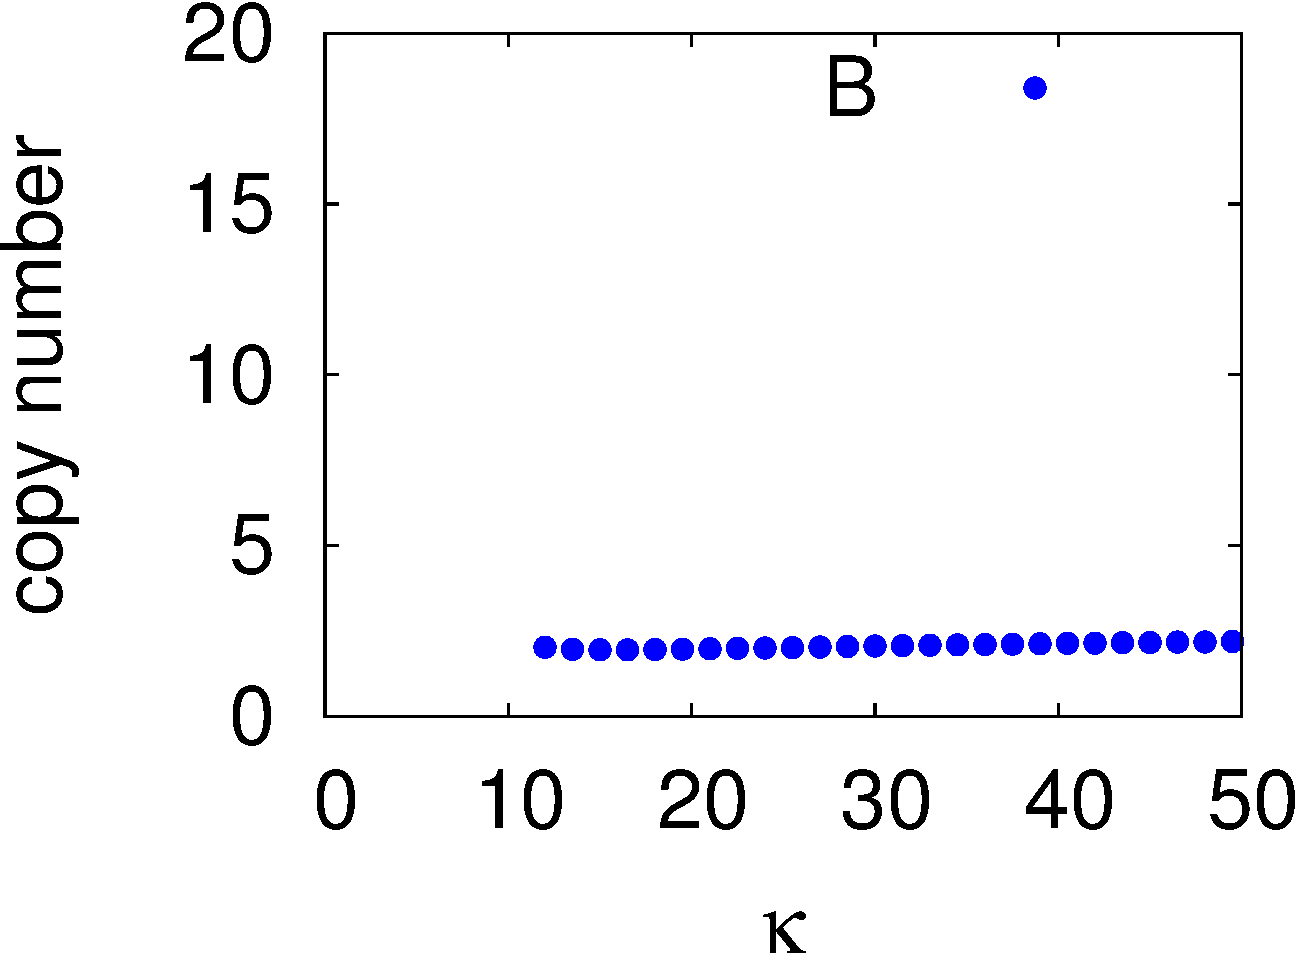
\includegraphics[width=\GGSIFixpointsPlotScale]{Figures-SI/FigureFixpointsWithFlux-B.pdf}
    \label{Fig-GG-SI-StabAnalysisWithFlux-2D-B}
  }\\
  \GGSIFixpointsPlotHspace
  \subfigure[][]{
    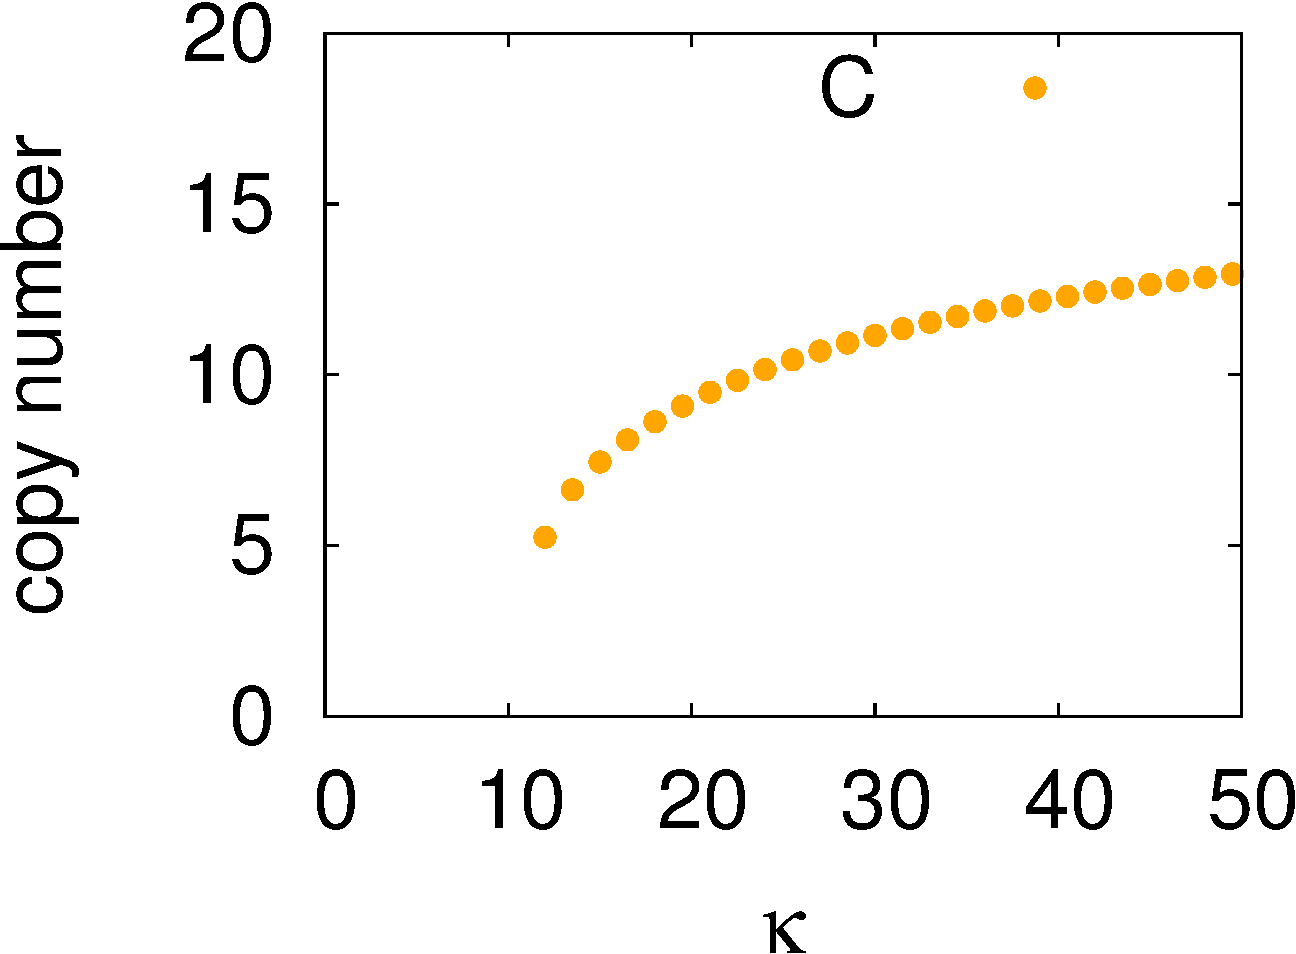
\includegraphics[width=\GGSIFixpointsPlotScale]{Figures-SI/FigureFixpointsWithFlux-C.pdf}
    \label{Fig-GG-SI-StabAnalysisWithFlux-2D-C}
  }
  \GGSIFixpointsPlotHspace\GGSIFixpointsPlotHspace
  \subfigure[][]{
    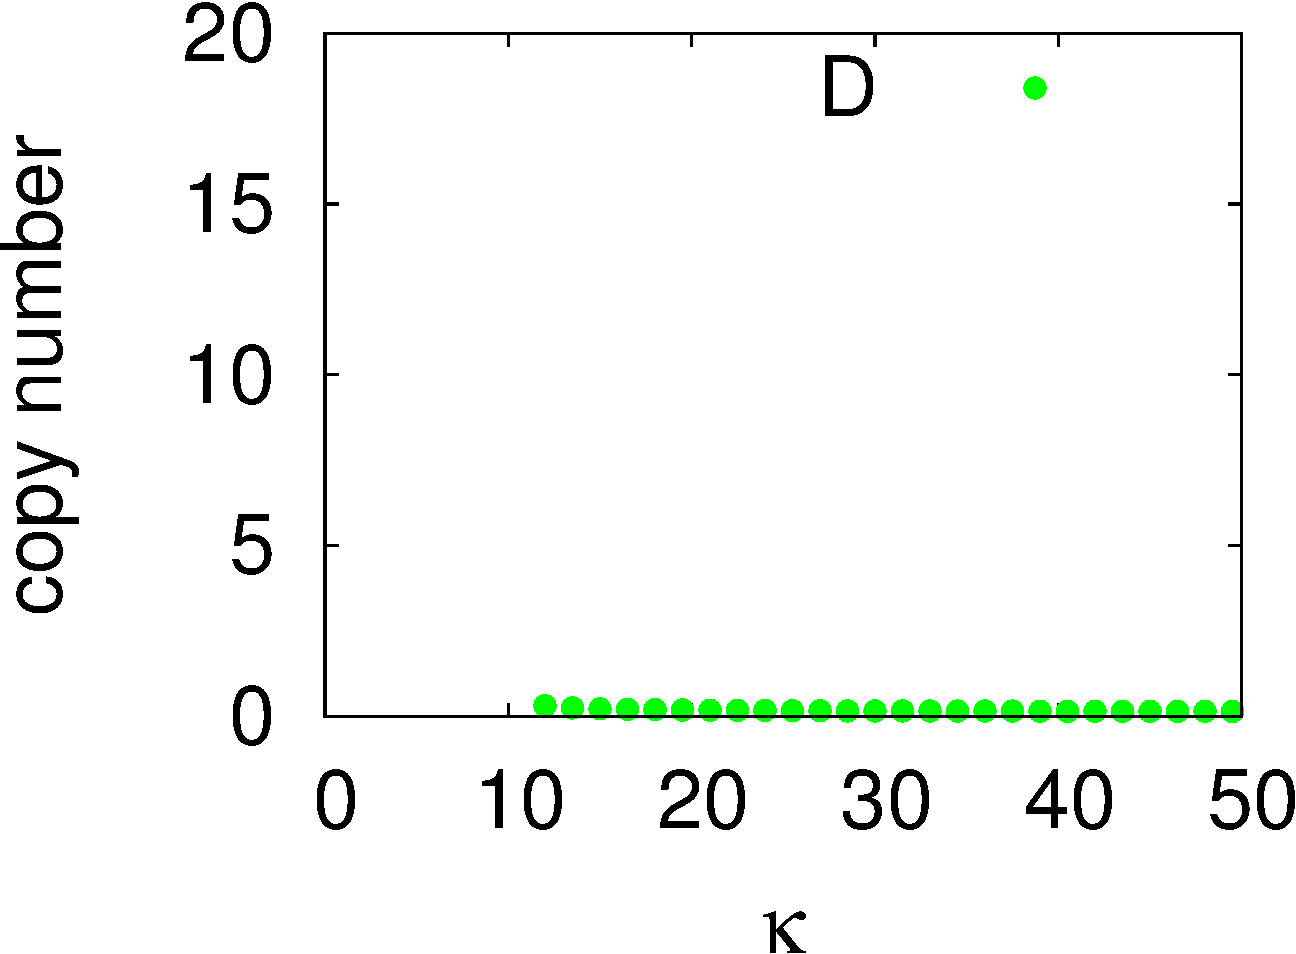
\includegraphics[width=\GGSIFixpointsPlotScale]{Figures-SI/FigureFixpointsWithFlux-D.pdf}
    \label{Fig-GG-SI-StabAnalysisWithFlux-2D-D}
  }
  \caption{\textbf{Steady state stability analysis with zero dimer fluxes.}
    Shown are the projected single components of stable fixed point solutions
    ${\rm (A,B,C,D)}$ for the total copy numbers (monomers + dimers)
    of the considered mutually repressing four-gene system as a function of $\kappa$,
    the ratio between weak and strong repressor off-rate,
    for the well-mixed system (A-D) and for the system with fluxes (E-H),
    mimicking the situation at an interface nucleus in the simulations.   
  \label{Fig-GG-SI-StabAnalysis-2D}
}
\end{figure}

\end{comment}


\newpage
%%%%%%%%%%%%%%%%
%%% TABLE S1 %%%
%%%%%%%%%%%%%%%%
\captionsetup[table]{width=.6\textwidth}
\mbox{} \vfill
\begin{table}[H]
 \centering
 \begin{tabular}{|l|c|lr|}
  \hline
  Quantity & Symbol & Value & Unit\\
  \hline
  \textit{Geometry} &&&\\
  Nuclear radius		& $r_N$		& 2.5	& $\mum$ \\
  Nuclear volume		& $V_N$		& 65.4	& $\mum^3$ \\
  No. of nuclei in axial direction		& $N_z$		& 40	& \\
  - resulting system length			& $L$		& 340	& $\mum$ \\
  No. of nuclei in circumferential direction	& $N_\phi$	& 8	& \\  
  \hline
  \textit{Production / degradation} &&&\\
  Protein production rate	& $\beta$	& 0.20 	& $\unit{s^{-1}}$ \\
  Monomer degradation rate	& $\mu_M$	& 0.05 	& $\unit{s^{-1}}$ \\
  Dimer degradation rate	& $\mu_D$	& 0.005 & $\unit{s^{-1}}$ \\
  - resulting effective degr. rate & $\mu_{eff}$	& 0.0095 & $\unit{s^{-1}}$ \\
  \hline
  \textit{Binding / unbinding} &&&\\
  Intranuclear diffusion const. & $D_N$		& 3.2	& $\mum^2/s$\\
  Repressor target site radius	& $\sigma_R$	& 0.5	& $\mum$ \\    
  - resulting (diff. ltd.) repressor on-rate 	& $\kRon$	& 20.1	& $\mum^3/s$ \\
  Standard (strong) repressor off-rate		& $\kRoffS$	& 0.06 	& $\unit{s^{-1}}$ \\
  Weak repressor off-rate			& $\kRoffW$	& varied & $\geq k^{\rm R,s}_{off}$ \\
  Monomer protein radius			& $\sigma_M$	& 0.05  & $\mum$ \\
  - resulting (diff. ltd.) dimerization forward rate & $\kDon$	& 4.0	& $\mum^3/s$ \\
  Dimerization backward rate			& $\kDoff$	& 0.062	& $\mum^3/s$ \\
  \hline
  \textit{Internuclear diffusion} &&&\\
  Standard internuclear diffusion const.	& $D$	& 1.0	& $\mum^2/s$ \\
  Internuclear lattice distance			& $l$	& 8.5	& $\mum$ \\
  \hline
 \end{tabular}

 \caption{The standard parameters of the simulated model of four mutually repressing genes
  prearranged in the ``alternating cushions'' pattern on a cylindrical lattice of expressing
  nuclei.
  \label{Tab-GG-SI-Parameters}
}
\end{table}
\vfill \mbox{}
\captionsetup[table]{width=\textwidth}



\newpage
%%%%%%%%%%%%%%%%%
%%% FIGURE S1 %%%
%%%%%%%%%%%%%%%%%
\newcommand{\PromA}{P^{\rm A}}
\newcommand{\kOn}{$\alpha$}
\newcommand{\kOffS}{$\sigma$}
\newcommand{\kOffW}{$\omega$}

\newcommand{\Adim}{{\rm A_2}}
\newcommand{\Bdim}{{\rm B_2}}
\newcommand{\Cdim}{{\rm C_2}}
\newcommand{\Ddim}{{\rm D_2}}
\newcommand{\Xdim}{{\rm X_2}}

\begin{figure}[H]
 \centering
 \begin{tikzpicture}[align=center, xscale=1.9, yscale=1.9]
 \node[draw,rectangle] (P0) at (0,6)   {$\PromA$};

 \node[draw,rectangle] (A)  at (2,6)   {${\rm A}$};
 \node[draw,rectangle] (A2) at (3,6)   {$\Adim$};

 \node                 (NIL) at (2.5,5) {$\varnothing$};

 \node[draw,rectangle] (PB) at (-2,4)  {$\PromA_{\Bdim}$};
 \node[draw,rectangle] (PC) at (0,4)   {$\PromA_{\Cdim}$};
 \node[draw,rectangle] (PD) at (2,4)   {$\PromA_{\Ddim}$};

 \node[draw,rectangle] (PBDl) at (-3,2) {$\PromA_{\Bdim\Ddim}$};
 \node[draw,rectangle] (PBC)  at (-1,2) {$\PromA_{\Bdim\Cdim}$};
 \node[draw,rectangle] (PCD)  at (1,2)  {$\PromA_{\Cdim\Ddim}$};
 \node[draw,rectangle] (PBDr) at (3,2)  {$\PromA_{\Bdim\Ddim}$};

 \node[draw,rectangle] (PBCD) at (0,-1)  {$\PromA_{\Bdim\Cdim\Ddim}$};

 % TOP LEVEL (4) TO LEVEL 3
 \draw[-latex] (P0) to[bend right=7] node[left=0.1cm]  {\kOn $[\Bdim]$}	(PB);
 \draw[-latex] (PB) to[bend right=7] node[below=0.3cm] {\kOffS}   	(P0);
 \draw[-latex] (P0) to[bend right=7] node[left]  {\kOn $[\Cdim]$}		(PC);
 \draw[-latex] (PC) to[bend right=7] node[right] {\kOffW}  		(P0);
 \draw[-latex] (P0) to[bend right=7] node[below=0.3cm]  {\kOn $[\Ddim]$}	(PD);
 \draw[-latex] (PD) to[bend right=7] node[right] {\kOffW}		(P0);

 % LEVEL 3 TO LEVEL 2
 \draw[-latex] (PB)   to[bend right=7] node[left]  {\kOn $[\Ddim]$} 	(PBDl);
 \draw[-latex] (PBDl) to[bend right=7] node[right] {\kOffW}		(PB);
 \draw[-latex] (PB)   to[bend right=7] node[left]  {\kOn $[\Cdim]$}	(PBC); 
 \draw[-latex] (PBC)  to[bend right=7] node[right] {\kOffW}		(PB);

 \draw[-latex] (PC)   to[bend right=7] node[left]  {\kOn $[\Ddim]$}	(PCD);
 \draw[-latex] (PCD)  to[bend right=7] node[right] {\kOffW}		(PC);
 \draw[-latex] (PC)   to[bend right=7] node[left]  {\kOn $[\Bdim]$} 	(PBC); 
 \draw[-latex] (PBC)  to[bend right=7] node[right] {\kOffS}		(PC);

 \draw[-latex] (PD)   to[bend right=7] node[left]  {\kOn $[\Bdim]$}	(PBDr);
 \draw[-latex] (PBDr) to[bend right=7] node[right] {\kOffS}		(PD);
 \draw[-latex] (PD)   to[bend right=7] node[left]  {\kOn $[\Cdim]$}	(PCD); 
 \draw[-latex] (PCD)  to[bend right=7] node[right] {\kOffW}		(PD);

 % LEVEL 2 TO BASE LEVEL (1)
 \draw[-latex] (PBDl) to[bend right=20] node[left=0.1cm] {\kOn $[\Cdim]$} (PBCD);
 \draw[-latex] (PBCD) to[bend right=-10] node[right] {\kOffW}		(PBDl);
 \draw[-latex] (PBC)  to[bend right=7] node[left]  {\kOn $[\Ddim]$}	(PBCD); 
 \draw[-latex] (PBCD) to[bend right=7] node[right] {\kOffW}		(PBC);

 \draw[-latex] (PCD)  to[bend right=7] node[left]  {\kOn $[\Bdim]$}	 (PBCD);
 \draw[-latex] (PBCD) to[bend right=7] node[right] {\kOffS}		 (PCD);
 \draw[-latex] (PBDr) to[bend right=-10] node[left=0.1cm] {\kOn $[\Cdim]$} (PBCD); 
 \draw[-latex] (PBCD) to[bend right=20] node[right] {\kOffW}		 (PBDr);

 % Equality between PBDl and PBDr
 \draw[loosely dashed] (PBDl) to[bend right=20] node[below] {$=$}	(PBDr);

 % Production from P0
 \draw[-latex] (P0) to node[above] {$\beta$} (A);
 \draw[-latex] (A)  to[bend left=10] node[above] {$\delta$} (A2);
 \draw[-latex] (A2) to[bend left=10] node[below] {$\epsilon$} (A);

 \draw[-latex] (A)  to node[left]  {$\mu_M$} (NIL);
 \draw[-latex] (A2) to node[right] {$\mu_D$} (NIL);

 \end{tikzpicture}

\caption{\textbf{Reaction network.} This schematic shows the set of reactions that affect production and degradation of a single
	gap gene species A. The strong repressor of A is denoted by B, the weak interaction partners by C and D. For each
        species, X denotes the monomer, $\Xdim$ the dimer. For easy readability here we abbreviate:
        $\alpha \equiv \kRon =$ diffusion limited repressor binding rate;
	$\sigma \equiv \kRoffS =$ next-nearest neighbor / strong repressor unbinding rate;
	$\omega \equiv \kRoffW =$ nearest-neighbor / weak repressor unbinding rate;
        $\delta \equiv \kDon =$ dimerization forward rate;
	$\epsilon \equiv \kDoff =$ dimerization backward rate.
	The schematic shows the reactions for the promoter of species A and
    its protein products, which we denote by ${\rm \left(A \vert\vert B,C,D\right)}$, 
    but holds similarly for all other combinations of regulated and regulating species,
    ${\rm \left(B \vert\vert A,C,D\right)}$,  ${\rm \left(C \vert\vert A,B,D\right)}$
    and ${\rm \left(D \vert\vert A,B,C\right)}$.
	\label{Fig-GG-SI-ReactionNetwork}
}
\end{figure}





%\section*{References}
% The bibtex filename
% \bibliography{GapGenes}

% \newpage
% \section*{Figure Legends}



%\section*{Tables}
%\begin{table}[!ht]
%\caption{
%\bf{Table title}}
%\begin{tabular}{|c|c|c|}
%table information
%\end{tabular}
%\begin{flushleft}Table caption
%\end{flushleft}
%\label{tab:label}
% \end{table}

\end{document}

